\chapter{Experimental Evaluation} \label{chap:results}
In this chapter the methods introduced in previous sections are evaluated and results are presented. In \cref{sec:verification_of_nn} the implemented classification framework called \textit{kitt\_nn} (see \cref{chap:kitt_nn} and details in \cref{sec:implementation_of_nn}) is verified by comparing to a publicly provided framework. Results of the developed pruning algorithm are shown in \cref{sec:pruning_algorithm_results}. Then, the overall terrain classification process is gradually evaluated in \cref{sec:terrain_processing_results}.

\section{Verification of the Network Implementation} \label{sec:verification_of_nn}
Classification performance of the implemented method \textit{kitt\_nn} is compared to a \textit{Scikit-neuralnetwork} classifier (\citep{misc:sknn}) presented in \cref{ssec:sknn}. The evaluation is performed on two datasets introduced in \cref{ssec:testing_datasets}.

The following \cref{fig:kitt_verify_acc} shows the progress of classification accuracy within learning epochs. For each dataset/framework combination, $ 10 $ observations were performed and mean values with standard deviation ranges are shown.

\begin{figure}[H]
  \centering
  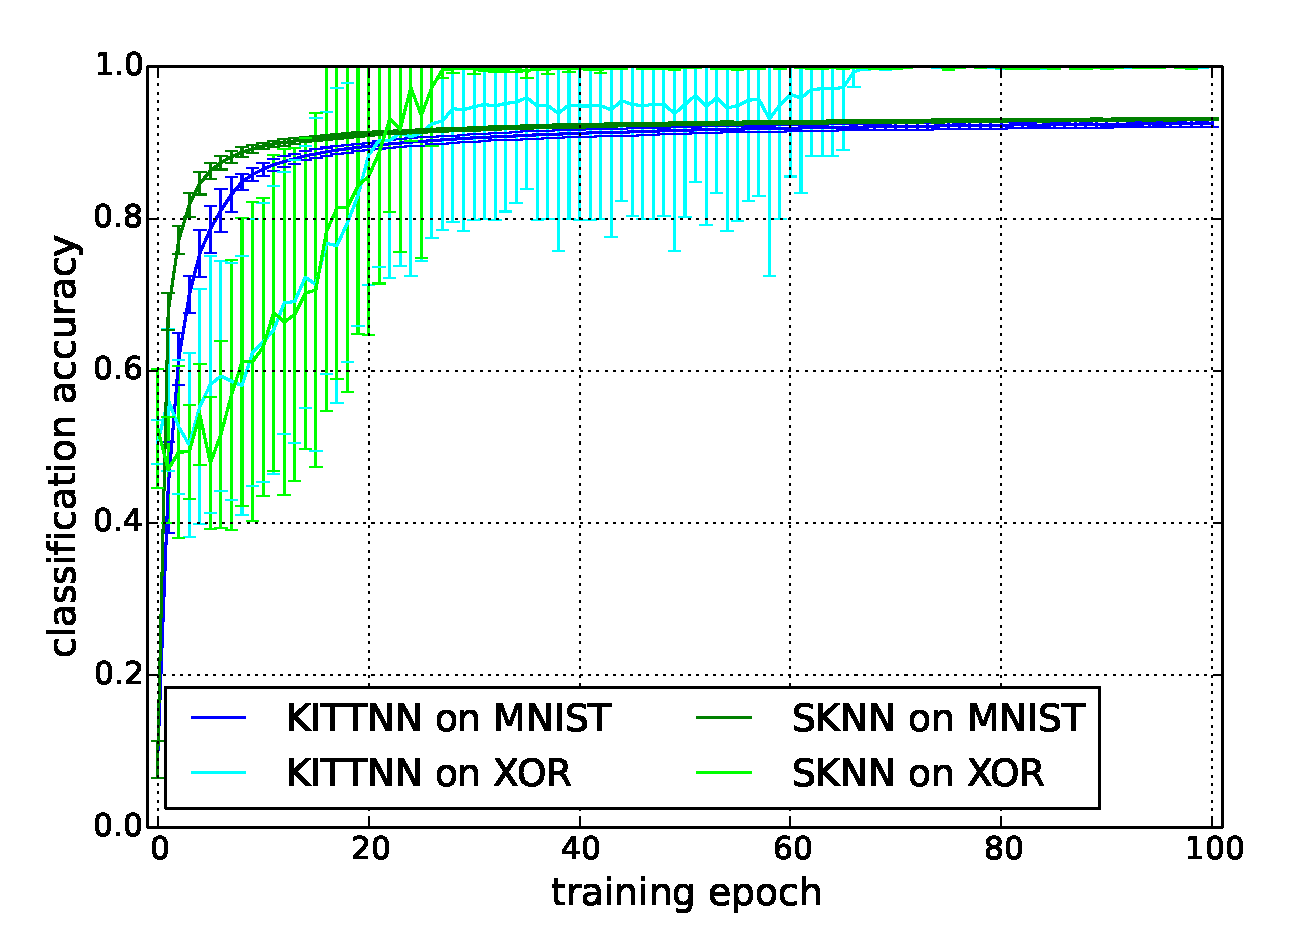
\includegraphics[width=0.8\textwidth]{kitt_verify_acc}
  \caption{Learning process compared to another framework (Scikit-neuralnetwork (sknn): \citep{misc:sknn}).}
  \label{fig:kitt_verify_acc}
\end{figure}

Regarding the XOR dataset, both nets start with the accuracy of about $ 0.5 $, as it has $ 2 $ classes and, naturally, with accuracy of about $ 0.1 $ for the $ 10 $ classes of the MNIST dataset. Individual observations differ more to each other (see the standard deviation in \cref{fig:kitt_verify_acc}) for XOR, as there are much less training samples compared to MNIST (50 times less). However, both nets are able to reach the accuracy of $ 1.0 $ on XOR within $ 100 $ epochs.

%\begin{figure}[H]
%  \centering
%  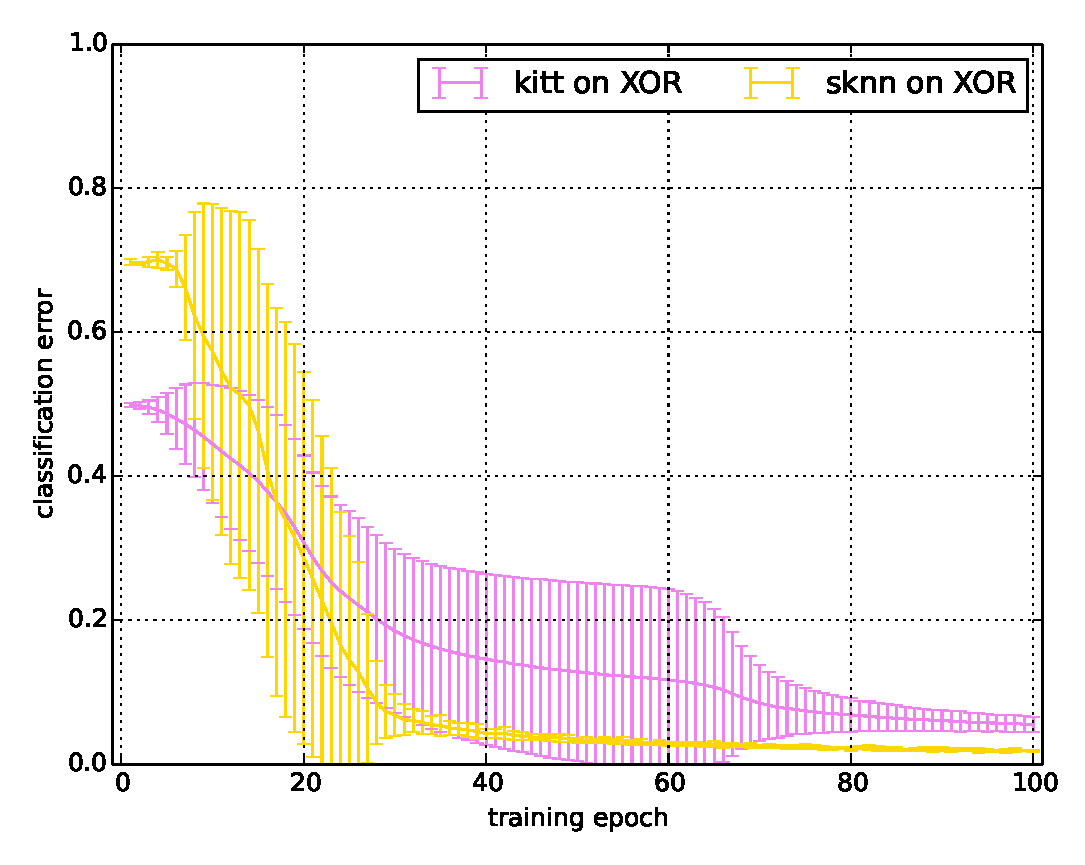
\includegraphics[width=0.8\linewidth]{kitt_verify_err}
%  \caption{Comparison of error through learning epochs to another framework (sknn).}
%  \label{fig:kitt_verify_err}
%\end{figure}

In \cref{tab:kitt_verify_f1}, the \textit{f1-score} measure (see \cref{eq:f1_score} in \cref{ssec:evaluation_methods}) is shown for individual classes (digits) of the MNIST dataset. This evaluation is done on the testing data.

\begin{table}[H]
\centering
\caption{Comparison of f1-score on MNIST to another framework (sknn)}
\label{tab:kitt_verify_f1}
\resizebox{\textwidth}{!} {
\begin{tabular}{|c|c|c|c|c|c|c|c|c|c|c|c|}
\hline
\textit{net}  & \textit{0} & \textit{1} & \textit{2} & \textit{3} & \textit{4} & \textit{5} & \textit{6} & \textit{7} & \textit{8} & \textit{9} & \textit{avg}  \\ \hline
\textbf{kitt} & 0.94       & 0.98       & 0.91       & 0.90       & 0.93       & 0.89       & 0.93       & 0.93       & 0.90       & 0.91       & \textbf{0.92} \\ \hline
\textbf{sknn} & 0.96       & 0.97       & 0.92       & 0.91       & 0.93       & 0.89       & 0.94       & 0.93       & 0.90       & 0.91       & \textbf{0.93} \\ \hline
\end{tabular}
}
\end{table}

In \cref{fig:kitt_verify_time}, a comparison of average epoch processing time is shown. The \textit{sknn} library provides an option to use \textit{gpu} in order to decrease the training time, hence also this training variant is included to the comparison.

This evaluation is done on the MNIST dataset only, as the training is quite fast on XOR for both implementations due to the smaller amount and size of samples. The average is computed out of $ 1000 $ samples, as we train $ 100 $ epochs in $ 10 $ observations.

\begin{figure}[H]
  \centering
  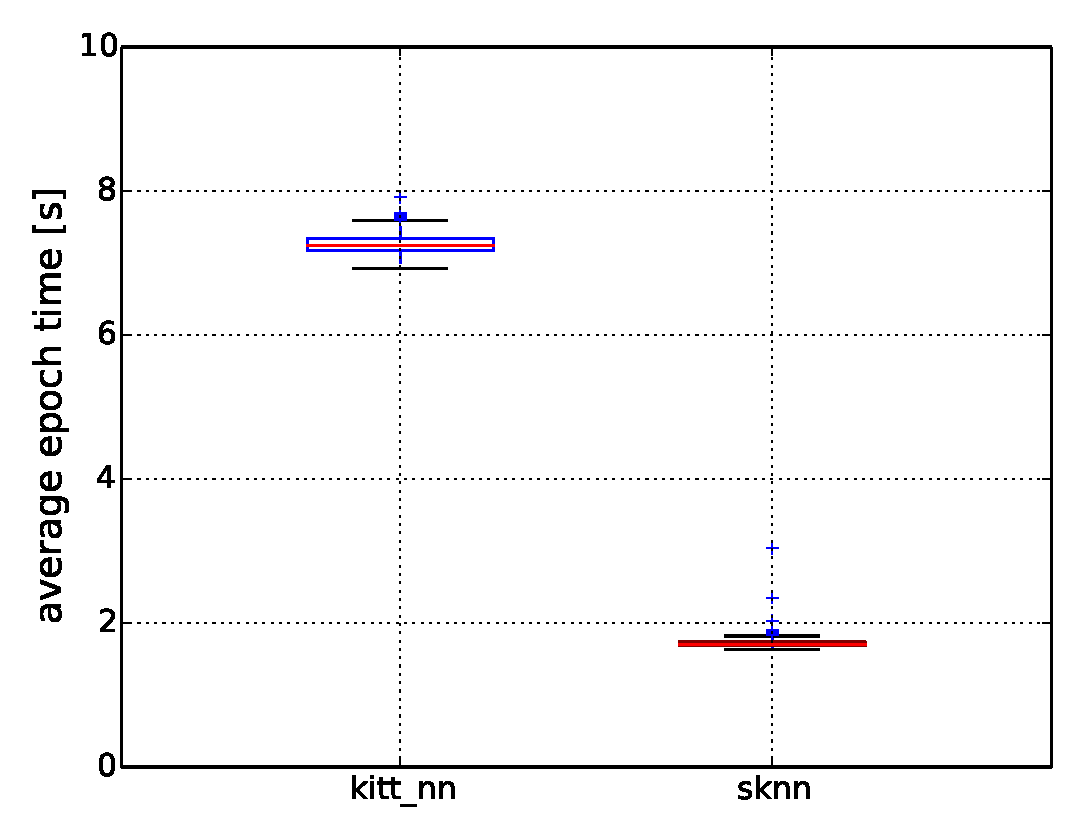
\includegraphics[width=0.8\linewidth]{kitt_verify_time}
  \caption{Comparison of average epoch processing time (1000 samples) to another framework (Scikit-neuralnetwork (sknn): \citep{misc:sknn}), MNIST dataset}
  \label{fig:kitt_verify_time}
\end{figure}

The implemented \textit{kitt\_nn} framework cannot compete in speed with the optimized stochastic \textit{GDA} of \textit{sknn} library. However, importantly for this study, the classification abilities have been verified.

\section[Performance Evaluation of the Pruning Algorithm]{Performance Evaluation of the Pruning \\Algorithm} \label{sec:pruning_algorithm_results}
This section presents results of the implemented pruning algorithm (introduced in \cref{sec:network_pruning_algorithm}). The input of the algorithm is given by a dataset and an obviously oversized neural network with a fully-connected structure. On the output, a pruned network of a minimal structure, but keeping a required classification accuracy, is expected.

The evalutaion of the algorithm is performed on the two datasets, XOR and MNIST, described in \cref{ssec:testing_datasets}.

\subsection{Evaluation on XOR Dataset} \label{ssec:evaluation_on_xor}
The XOR dataset is essential for testing the functionality of the algorithm, as we know the minimal network structure for this problem ($ [2, 2, 1] $). Initially, a network with one hidden layer of $ 100 $ neurons is constructed as the algorithm input (\cref{img:pa_xor_start}). The desired structure is shown in \cref{img:pa_xor_final}.

During the pruning process, three key network properties are observed:
\begin{enumerate}
\item network structure;
\item number of synapses in the network;
\item classification accuracy on a chosen dataset.
\end{enumerate}

Those are shown with respect to the pruning step (see the pruning loop in \cref{img:pruning_algorithm}) all together in \cref{fig:pa_result_xor}.

\begin{figure}[H]
  \centering
  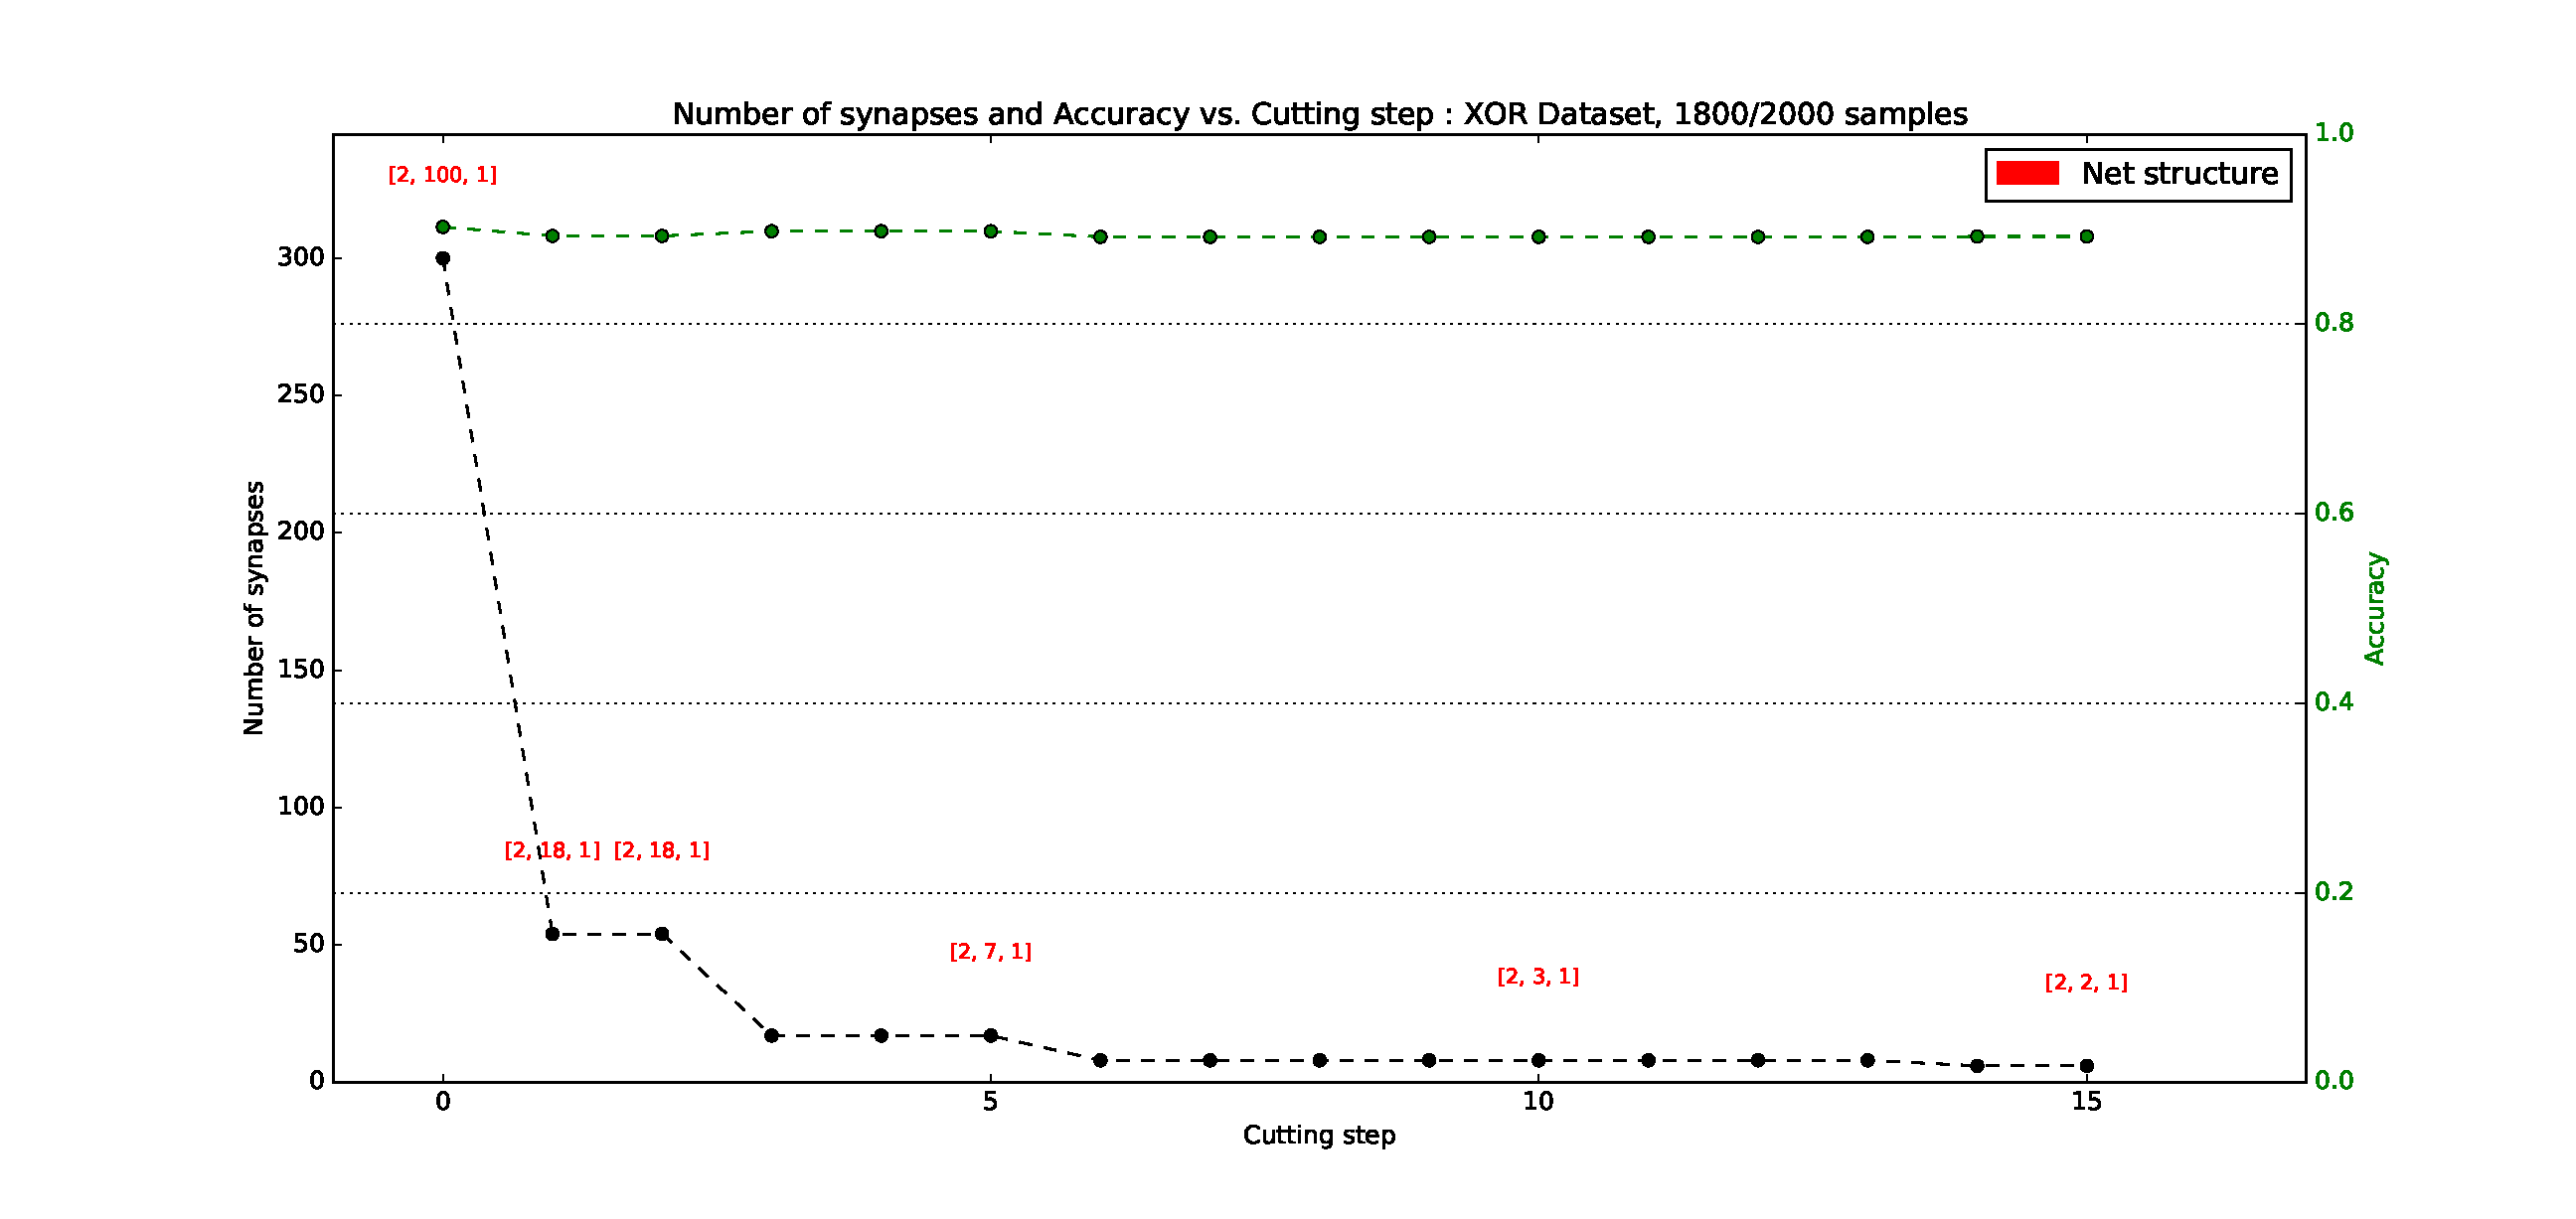
\includegraphics[width=1.0\textwidth]{pa_result_xor}
  \caption{Results of the pruning algorithm on XOR dataset.}
  \label{fig:pa_result_xor}
\end{figure}

The results are obtained by averaging $ 10 $ observations, so they are not dependent on initial conditions. For retraining the network after a pruning step, training data is used. For verification, whether the network is capable of classification, validation data is used. Testing data is used to check the accuracy after pruning (values in \cref{fig:pa_result_xor}).

Algorithm parameters:
\begin{itemize}
\item initial network structure: $ [2, 100, 1] $
\item required classification accuracy on validation data: $ 0.9 $
\item learning rate: $ 0.5 $
\item percentile levels: $ [50, 20, 5, 0] $
\end{itemize}

Algorithm outcomes:
\begin{itemize}
\item pruning steps: $ 10 $
\item final strucuture: $ [2, 2, 1] $
\item number of removed synapses: $ 294 $ ($ 300 $ -> $ 6 $)
\item classification accuracy on testing data: $ 0.99 $
\end{itemize}

\begin{figure}[H]
\centering
\begin{subfigure}{0.45\textwidth}
  \centering
  \includegraphics[width=0.8\linewidth]{pa_xor_start.png}
  \caption{PA input: oversized and fully-connected network (XOR)}
  \label{img:pa_xor_start}
\end{subfigure}%
\begin{subfigure}{0.45\textwidth}
  \centering
  \includegraphics[width=0.8\linewidth]{pa_xor_final.png}
  \caption{PA output: minimal network structure (XOR)}
  \label{img:pa_xor_final}
\end{subfigure}
\caption{Application of the pruning algorithm on XOR}
\label{img:pa_xor_morph}
\end{figure}

\subsection{Evaluation on MNIST Dataset} \label{ssec:evaluation_on_mnist}
Similarly, the algorithm is evaluated on the MNIST dataset. In this case, the minimal structure is not known. The recommended size of the hidden layer for MNIST classification is $ 15 $. In \cref{fig:kitt_verify_acc} the classification accuracy of \textit{kitt\_nn} framework on this dataset is presented. Apparently, it is possible to reach a success rate around $ 90\% $. Hence these parameters are used:

\begin{itemize}
\item initial network structure: $ [784, 15, 10] $ ($ 784 $, because the samples are images of size $ 28x28 $, and $ 10 $, because we have ten digits)
\item required classification accuracy on validation data: $ 0.89 $
\item learning rate: $ 0.1 $
\item percentile levels: $ [50, 35, 20, 10, 5, 0] $
\end{itemize}

\cref{fig:pa_result_mnist} shows a significant reduction of synapses while the classification accuracy is kept on $ 0.89 $. The shown results are obtained by averaging $ 10 $ observations.
\begin{figure}[H]
  \centering
  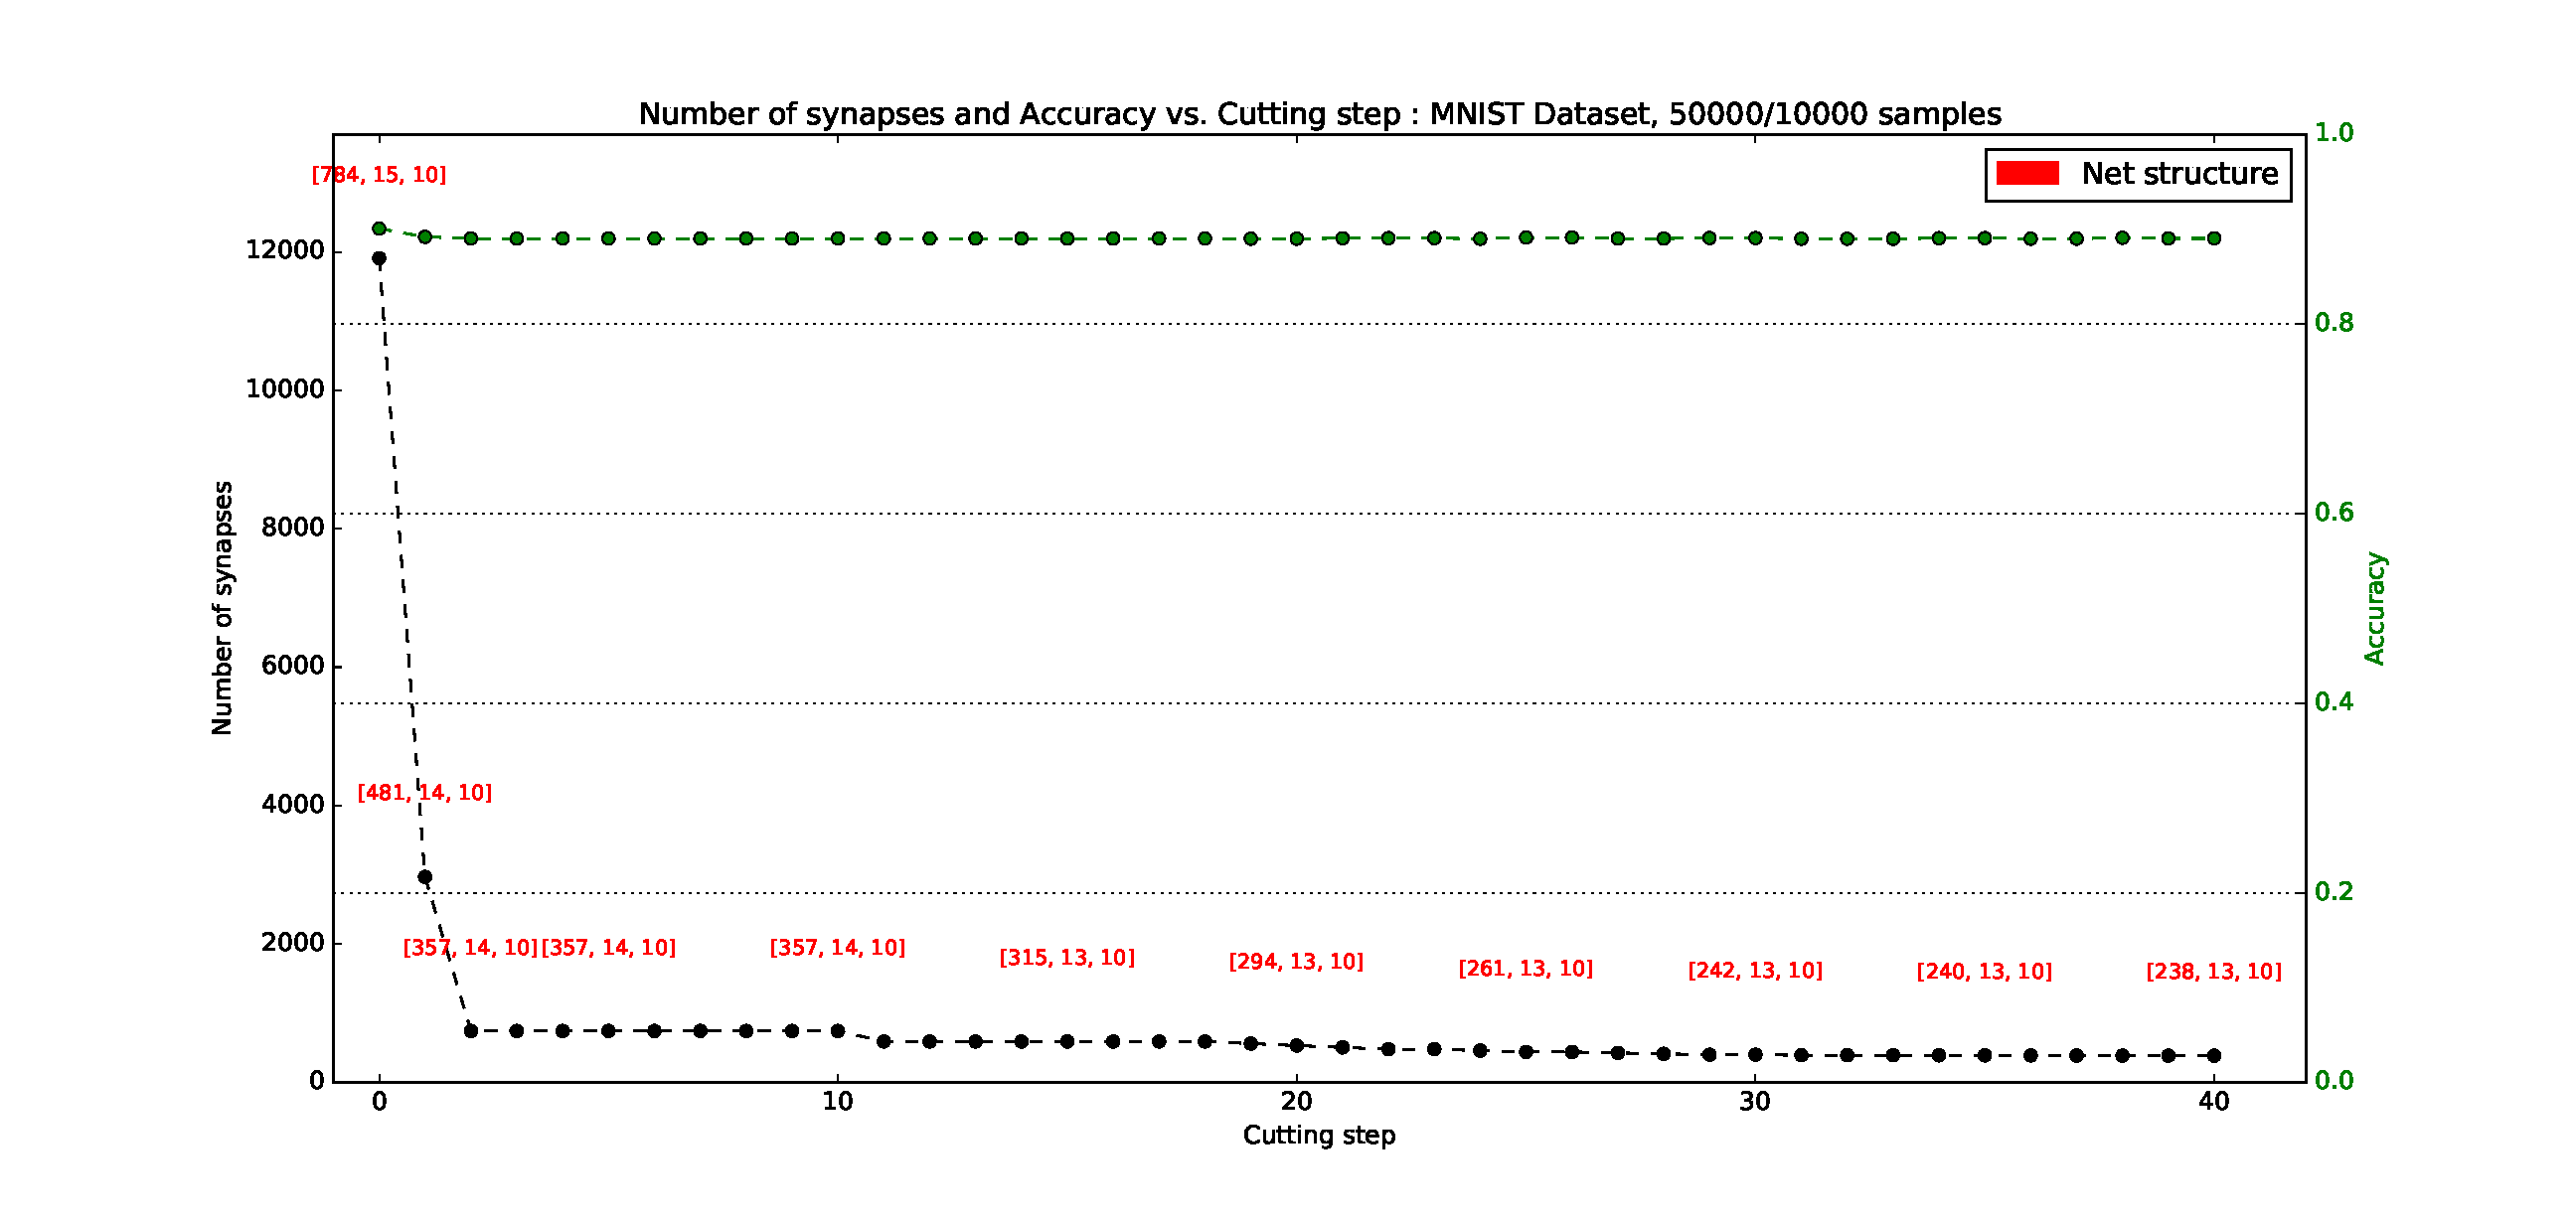
\includegraphics[width=1.0\textwidth]{pa_result_mnist}
  \caption{Pruning Algorithm Results on MNIST Dataset.}
  \label{fig:pa_result_mnist}
\end{figure}

Results of the pruning algorithm on MNIST:
\begin{itemize}
\item pruning steps: $ 76 $
\item final strucuture: $ [495, 15, 10] $
\item number of removed synapses: $ 11075 $ ($ 11910 $ -> $ 835 $ : $ 92.9\% $)
\item classification accuracy on testing data: $ 0.88776 $
\end{itemize}

The figure \ref{fig:pa_result_mnist} says that more than $ 90\% $ of the synapses in the initial network structure are redundant. Regarding the number of neurons in the network, mostly the input layer is reduced. These results make a pretty good sense, as shown in \cref{sssec:mnist_analysis}.

The following \cref{tab:pa_results_mnist} presents statistics of the first seven steps of one of the performed observations. For each step we can see the current percentile level (see \cref{img:pruning_algorithm}), corresponding reduction in the network and retraining results.

\begin{table}[H]
\centering
\caption{PA progress example on MNIST}
\label{tab:pa_results_mnist}
\resizebox{\textwidth}{!} {
\begin{tabular}{|l|c|c|c|c|c|c|c|c|}
\hline
\multicolumn{1}{|c|}{\textit{step}} & \textit{0 (initial)} & \textit{1}                  & \textit{2}                  & \textit{3}                  & \textit{4}                 & \textit{5} & \textit{6} & \textit{7} \\ \hline
percentile level                    & 50                   & 50                          & 50                          & 50                          & 50                         & 35         & 20           & 20           \\ \hline
synapses removed                    & X                    & 5955                        & 2978                        & 1489                        & 744                        & 521            & 298            & 238           \\ \hline
input neurons left                  & 784                  & 784                         & 769                         & 664                         & 464                        & 539           & 602           & 521           \\ \hline
synapses left                       & 11910                & 5955                        & 2977                        & 1488                        & 744                        & 967           & 1190           & 952           \\ \hline
acc. after pruning                  & X                    & 0.9                         & 0.887                       & 0.851                       &  0.817                      & 0.858            & 0.880           & 0.878           \\ \hline
retrained?                          & X                    & \cellcolor[HTML]{34FF34}yes & \cellcolor[HTML]{34FF34}yes & \cellcolor[HTML]{34FF34}yes & \cellcolor[HTML]{FD6864}no & \cellcolor[HTML]{FD6864}no            & \cellcolor[HTML]{34FF34}yes            & \cellcolor[HTML]{34FF34}yes            \\ \hline
epochs to retrain                   & X                    & 0                           & 4                           & 63                          & \textgreater 100           & \textgreater 100           & 8           & 12           \\ \hline
\end{tabular}
}
\end{table}

In this example, the algorithm uses the percentile level of $ 50 $ in the first three steps, meaning it cuts out the half of the synapses each time. In the fourth step, the network is not able to retrain after cutting half of the remaining synapses, hence the percentile level is decreased to $ 35 $ and less synapses are tried to be removed in the fifth step. However, the retraining is not successful again (the accuracy of $ 0.89 $ is not reached in $ 100 $ epochs), so the percentile level is decreased to $ 20 $. This time the pruned network is able to retrain, so a new structure is saved and the algorithm continues with the percentile level of $ 20 $ in the next steps.

The following figures (\ref{img:pa_mnist_morph}) illustrate the transformation of the network.
\begin{figure}[H]
\centering
\begin{subfigure}{0.45\textwidth}
  \centering
  \includegraphics[width=0.8\linewidth]{pa_mnist_start.png}
  \caption{PA input: oversized and fully-connected network (MNIST)}
  \label{img:pa_mnist_start}
\end{subfigure}%
\begin{subfigure}{0.45\textwidth}
  \centering
  \includegraphics[width=0.8\linewidth]{pa_mnist_final.png}
  \caption{PA output: minimal network structure (MNIST)}
  \label{img:pa_mnist_final}
\end{subfigure}
\caption{Application of the pruning algorithm on MNIST}
\label{img:pa_mnist_morph}
\end{figure}

\subsubsection{Minimal Structure in MNIST Dataset} \label{sssec:mnist_analysis}
As mentioned in \cref{ssec:minimal_structure_util}, minimal structures obtained from the pruning algorithm can be further researched.

For instance, considering the MNIST dataset, there is an image (meaning a vector of pixels) as the network input. As the output, there are $ 10 $ classes corresponding to digits. Having the minimal structure, one can find out which pixels are related to e.g. digit $ 7 $ class or which pixels are totally useless for classification.

\begin{figure}[H]
\centering
\begin{subfigure}{0.45\textwidth}
  \centering
  
\includegraphics[width=0.7\linewidth]{mnist_interesting_pixels.png}
  \caption{}
  \label{img:msu_interesting}
\end{subfigure}%
\begin{subfigure}{0.45\textwidth}
  \centering
  
\includegraphics[width=0.7\linewidth]{mnist_pixels_seven.png}
  \caption{}
  \label{img:msu_seven}
\end{subfigure}
\caption{Demonstration of the minimal structures utilization on MNIST; (A) Pixels of the MNIST samples that are essential for classification; (B) Pixels of the MNIST samples influencing the class $ 7 $}
\label{img:pa_xor_morph}
\end{figure}

As illustrated in \cref{img:structure_util}, paths from the input to the output layer can be tracked. This way we can find paths for every output neuron and see which input neurons are connected with it. \cref{img:msu_seven} shows in white all input neurons (pixels of the $ 28x28 $ input images) that are connected to output neuron $ 7 $.

In \cref{img:msu_interesting}, an analysis of all $ 784 $ input neurons is presented. As there are $ 15 $ hidden neurons, each input neuron can have maximally $ 15 $ connections and, naturally, minimially $ 0 $ connections in the final structure. 

The number of remaining connections $ n\_con $ is mapped into $ [0, 255] $ range, in order to be represented as a greyscale color, using the following equation:

\begin{align} \label{eq:grayscale_mapping}
intensity = \frac{255 \cdot n\_con}{15}
\end{align}

\cref{img:msu_interesting} shows the number of connections to the hidden layer $ n\_con $ as a greyscale value ($ intensity $) for every pixel of input samples. The more bright the pixel is, the more connections it has. Black pixels have no connections to the hidden layer and so they are not used for classification at all.

The results on both figures (\ref{img:msu_interesting} and \ref{img:msu_seven}) make a good sense, as the pixels close to borders are black. One could expect, that these pixels are not important, as the digits are centered in the images.

\section{Results of Terrain Classification} \label{sec:terrain_processing_results}
In this section, results of the overall terrain classification process are shown. The results are sorted in correspondance to the methods explanation in \cref{chap:terrain_classification}.

\subsection{Selection of Learning Parameters} \label{ssec:analysis_of_learning_parameters}

learning rate

\begin{figure}[H]
  \centering
  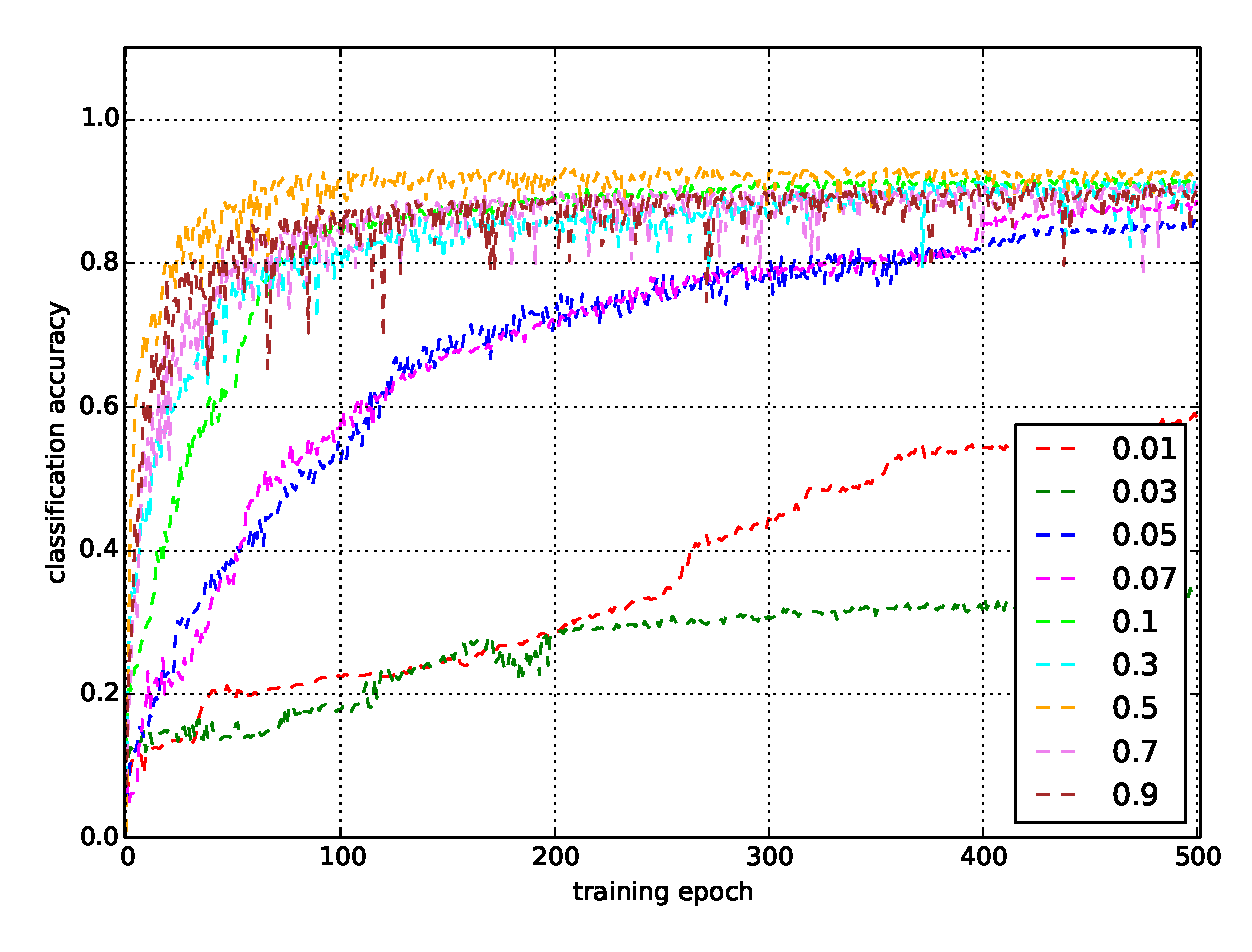
\includegraphics[width=0.8\textwidth]{cl_lr_vs_epoch_st20}
  \caption{Learning rate analysis. Net structure: [960, 20, 14].}
  \label{fig:lr_analysis}
\end{figure}

\begin{figure}[H]
  \centering
  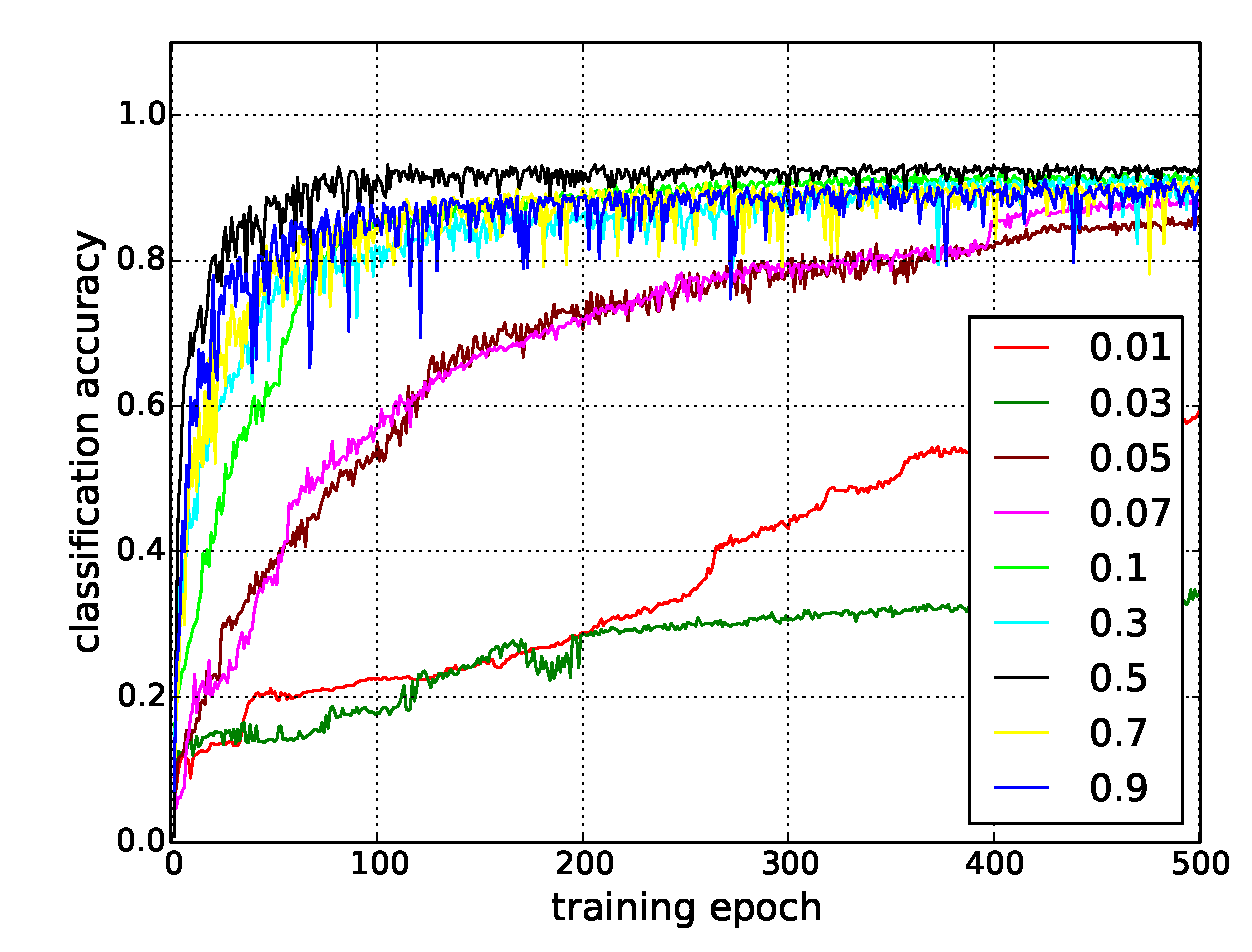
\includegraphics[width=0.8\textwidth]{cl_lr_vs_epoch_st20_example}
  \caption{Learning rate analysis. Net structure: [960, 20, 14].}
  \label{fig:lr_analysis_example}
\end{figure}

\begin{figure}[H]
  \centering
  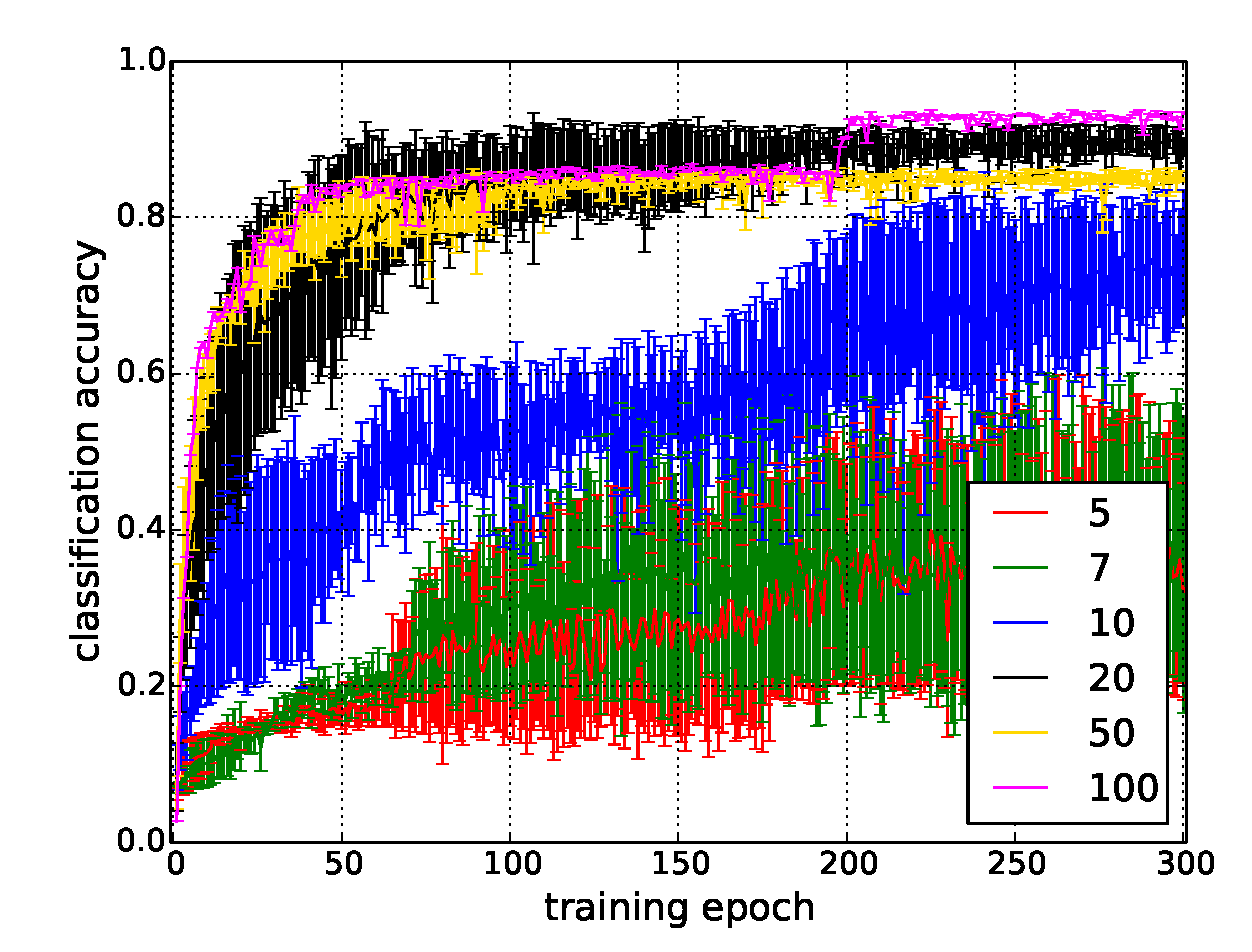
\includegraphics[width=0.8\textwidth]{cl_st_vs_epoch_lr05}
  \caption{Network structure analysis. Learning rate: 0.5.}
  \label{fig:st_analysis}
\end{figure}

\begin{figure}[H]
  \centering
  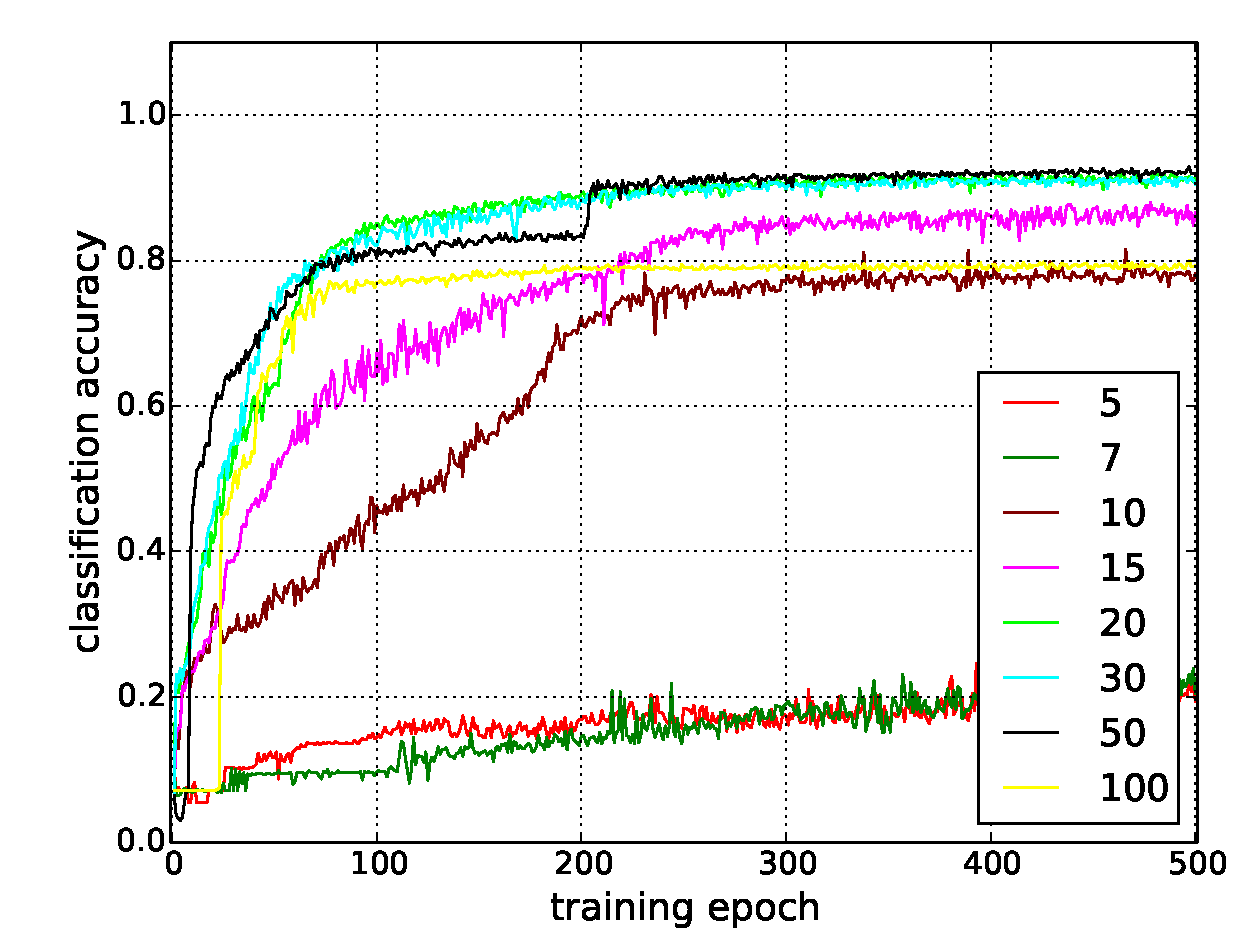
\includegraphics[width=0.8\textwidth]{cl_st_vs_epoch_lr05_example}
  \caption{Network structure analysis. Learning rate: 0.5.}
  \label{fig:st_analysis_example}
\end{figure}

\begin{figure}[H]
  \centering
  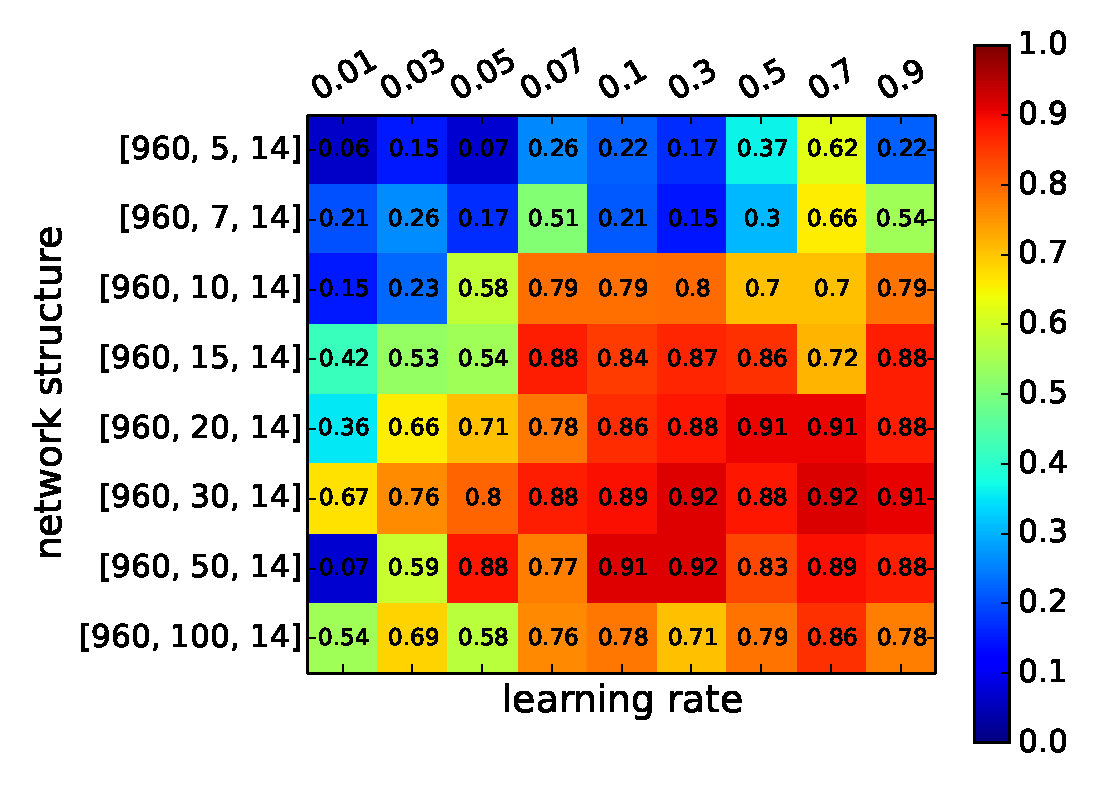
\includegraphics[width=1.0\textwidth]{cl_st_lr_mat}
  \caption{Learning parameters analysis: Classification accuracy vs. learning rate and network structure}
  \label{fig:acc_st_lr_mat}
\end{figure}

\subsection{Classification Performance} \label{ssec:classification_performance}

\begin{table}[H]
\centering
\caption{Classification results}
\label{tab:classification_results}
\resizebox{\textwidth}{!} {
\begin{tabular}{|c|c|c|c|c|c|c|}
\hline
\textit{dataset} & \textit{accuracy} & \textit{precision} & \textit{recall} & \textit{f1-score} & \textit{error} & \textit{ep. time {[}s{]}} \\
\hline
00\_00\_80\_p 	& 0.624 	& 0.596 	& 0.624 	& 0.576 	& 0.072 	& 1.089 	 \\ \hline
00\_00\_80\_a 	& 0.89 	& 0.888 	& 0.89 	& 0.878 	& 0.02 	& 1.33 	 \\ \hline
00\_03\_40\_a 	& 0.902 	& 0.9 	& 0.9 	& 0.9 	& 0.019 	& 0.765 	 \\ \hline
00\_00\_30\_a 	& 0.847 	& 0.84 	& 0.848 	& 0.842 	& 0.03 	& 0.964 	 \\ \hline
00\_00\_10\_p 	& 0.489 	& 0.468 	& 0.49 	& 0.43 	& 0.089 	& 0.565 	 \\ \hline
00\_01\_40\_a 	& 0.776 	& 0.79 	& 0.78 	& 0.76 	& 0.04 	& 0.751 	 \\ \hline
00\_00\_01\_a 	& 0.639 	& 0.646 	& 0.638 	& 0.624 	& 0.073 	& 0.526 	 \\ \hline
00\_00\_80\_t	& 0.761 	& 0.764 	& 0.76 	& 0.742 	& 0.051 	& 0.715 	 \\ \hline
00\_00\_20\_a 	& 0.85 	& 0.848 	& 0.85 	& 0.846 	& 0.03 	& 0.894 	 \\ \hline
00\_05\_40\_a 	& 0.884 	& 0.88 	& 0.88 	& 0.88 	& 0.019 	& 0.76 	 \\ \hline
00\_00\_40\_a 	& 0.906 	& 0.906 	& 0.906 	& 0.906 	& 0.019 	& 0.865 	 \\ \hline
00\_00\_10\_a 	& 0.805 	& 0.806 	& 0.804 	& 0.798 	& 0.04 	& 0.526 	 \\ \hline
00\_00\_40\_p 	& 0.696 	& 0.702 	& 0.694 	& 0.666 	& 0.06 	& 0.707 	 \\ \hline
00\_00\_10\_t 	& 0.423 	& 0.432 	& 0.424 	& 0.386 	& 0.102 	& 0.469 	 \\ \hline
00\_10\_40\_a 	& 0.851 	& 0.85 	& 0.85 	& 0.85 	& 0.026 	& 0.792 	 \\ \hline
00\_00\_40\_t	& 0.701 	& 0.692 	& 0.702 	& 0.67 	& 0.064 	& 0.475 	 \\ \hline
01\_03\_40\_a 	& 0.772 	& 0.78 	& 0.77 	& 0.76 	& 0.044 	& 1.314 	 \\ \hline
01\_10\_40\_a 	& 0.639 	& 0.67 	& 0.64 	& 0.63 	& 0.06 	& 0.944 	 \\ \hline
01\_01\_40\_a 	& 0.759 	& 0.77 	& 0.76 	& 0.75 	& 0.052 	& 1.093 	 \\ \hline
01\_00\_40\_a 	& 0.815 	& 0.83 	& 0.81 	& 0.82 	& 0.041 	& 0.844 	 \\ \hline
01\_05\_40\_a 	& 0.78 	& 0.79 	& 0.78 	& 0.77 	& 0.044 	& 0.9 	 \\ \hline
03\_10\_40\_a 	& 0.565 	& 0.53 	& 0.56 	& 0.54 	& 0.063 	& 0.946 	 \\ \hline
03\_05\_40\_a 	& 0.645 	& 0.64 	& 0.65 	& 0.63 	& 0.054 	& 0.871 	 \\ \hline
03\_00\_40\_a 	& 0.714 	& 0.73 	& 0.71 	& 0.7 	& 0.057 	& 0.831 	 \\ \hline
03\_03\_40\_a 	& 0.719 	& 0.74 	& 0.72 	& 0.72 	& 0.046 	& 0.939 	 \\ \hline
03\_01\_40\_a 	& 0.779 	& 0.78 	& 0.78 	& 0.78 	& 0.042 	& 1.068 	 \\ \hline
05\_01\_40\_a	& 0.732 	& 0.74 	& 0.73 	& 0.73 	& 0.052 	& 1.018 	 \\ \hline
05\_05\_40\_a 	& 0.651 	& 0.66 	& 0.65 	& 0.64 	& 0.056 	& 0.933 	 \\ \hline
05\_10\_40\_a 	& 0.601 	& 0.61 	& 0.6 	& 0.6 	& 0.062 	& 0.954 	 \\ \hline
05\_03\_40\_a 	& 0.677 	& 0.71 	& 0.68 	& 0.67 	& 0.052 	& 0.949 	 \\ \hline
05\_00\_40\_a 	& 0.685 	& 0.72 	& 0.69 	& 0.68 	& 0.055 	& 0.835 	 \\ \hline
10\_10\_40\_a 	& 0.459 	& 0.46 	& 0.46 	& 0.43 	& 0.087 	& 0.983 	 \\ \hline
10\_03\_40\_a	& 0.621 	& 0.63 	& 0.62 	& 0.6 	& 0.07 	& 0.824 	 \\ \hline
10\_01\_40\_a 	& 0.594 	& 0.63 	& 0.59 	& 0.58 	& 0.072 	& 1.131 	 \\ \hline
10\_00\_40\_a 	& 0.614 	& 0.61 	& 0.61 	& 0.59 	& 0.067 	& 0.822 	 \\ \hline
10\_05\_40\_a 	& 0.543 	& 0.58 	& 0.54 	& 0.53 	& 0.074 	& 0.875 	 \\ \hline
20\_01\_40\_a 	& 0.459 	& 0.48 	& 0.46 	& 0.44 	& 0.093 	& 1.071 	 \\ \hline
20\_00\_40\_a 	& 0.463 	& 0.47 	& 0.46 	& 0.44 	& 0.087 	& 0.827 	 \\ \hline
20\_05\_40\_a 	& 0.436 	& 0.45 	& 0.44 	& 0.41 	& 0.091 	& 0.947 	 \\ \hline
20\_10\_40\_a 	& 0.371 	& 0.36 	& 0.37 	& 0.36 	& 0.09 	& 0.993 	 \\ \hline
20\_03\_40\_a	& 0.439 	& 0.47 	& 0.44 	& 0.42 	& 0.091 	& 0.923 	 \\ \hline
\end{tabular}
}
\end{table}

\subsection{Influence of Noise on Classification} \label{ssec:final_configuration}

\begin{figure}[H]
  \centering
  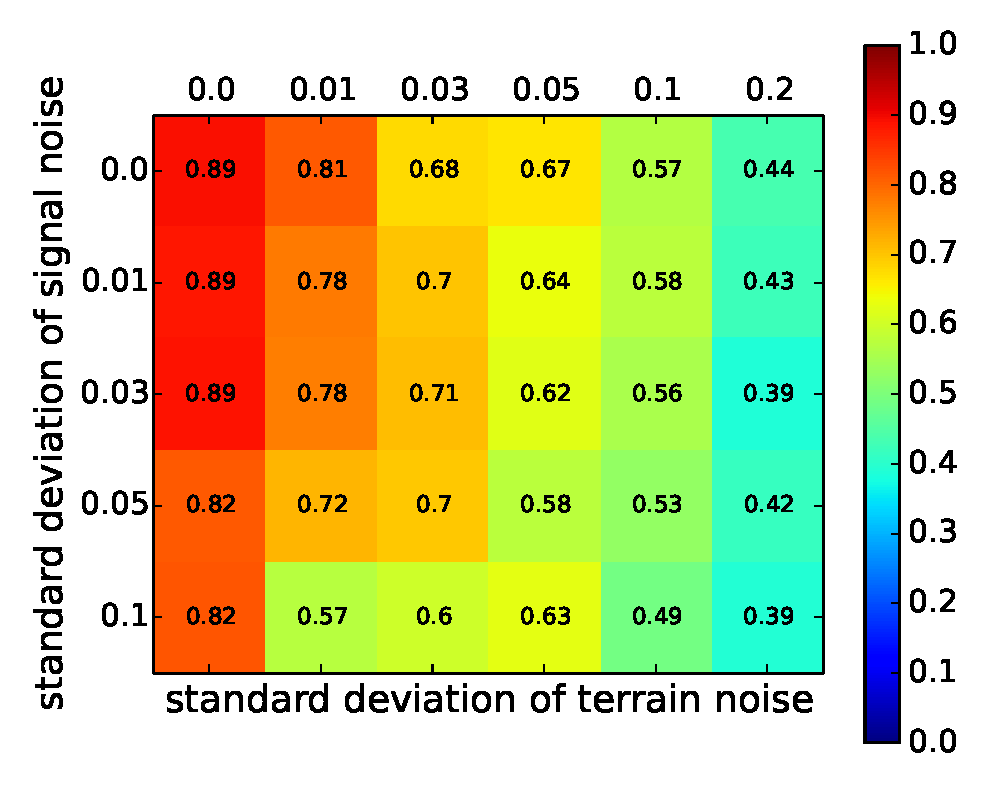
\includegraphics[width=1.0\textwidth]{cl_acc_tn_sn_mat}
  \caption{Additive terrain and signal noise: influence on the accuracy}
  \label{fig:acc_tn_sn_mat}
\end{figure}

\subsection{Time Needed for Classification} \label{ssec:number_of_timesteps}

\begin{figure}[H]
  \centering
  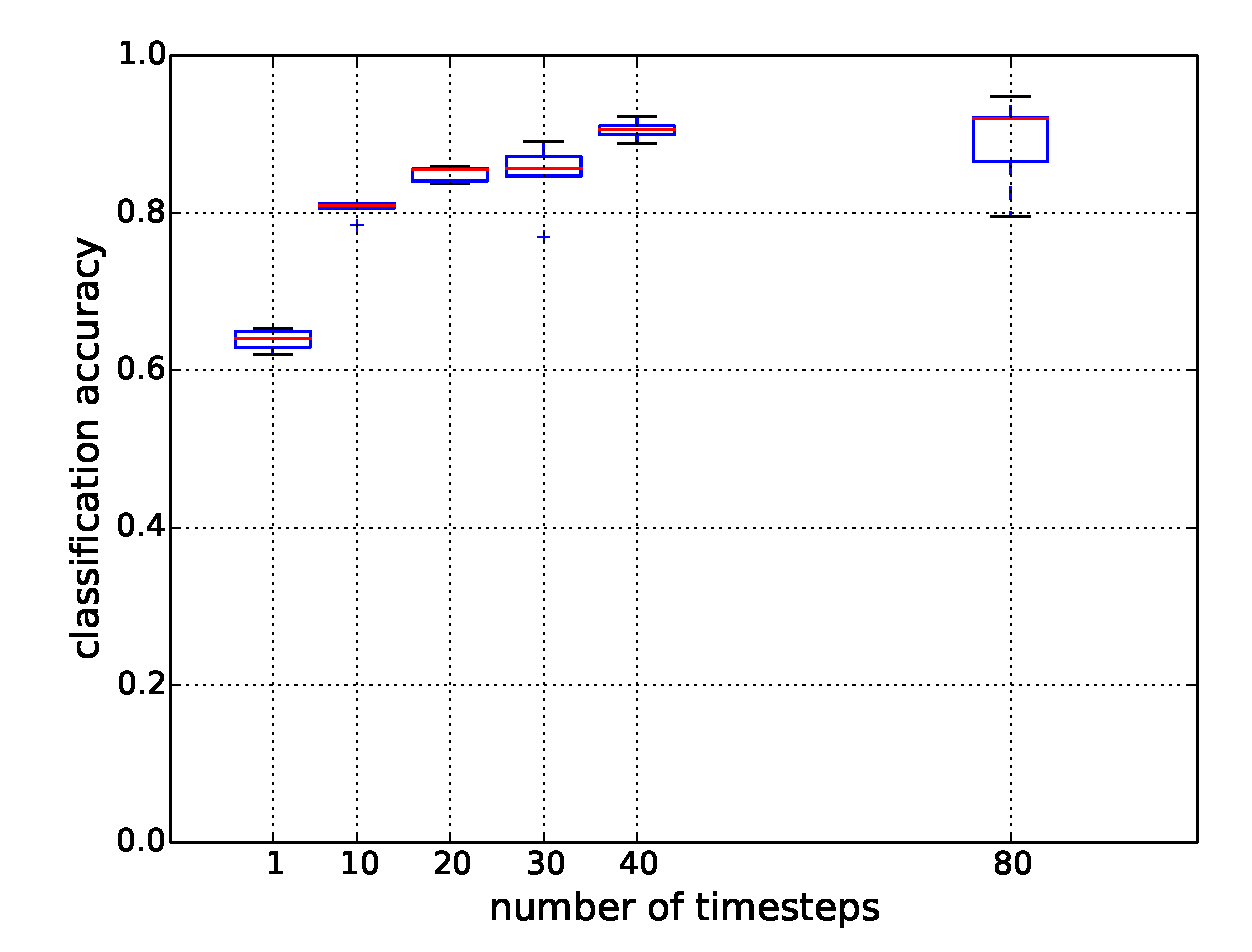
\includegraphics[width=1.0\textwidth]{cl_ts_acc_boxplot}
  \caption{Number of simulation timesteps: influence on the accuracy and training time}
  \label{fig:ts_acc_boxplot}
\end{figure}

\begin{figure}[H]
  \centering
  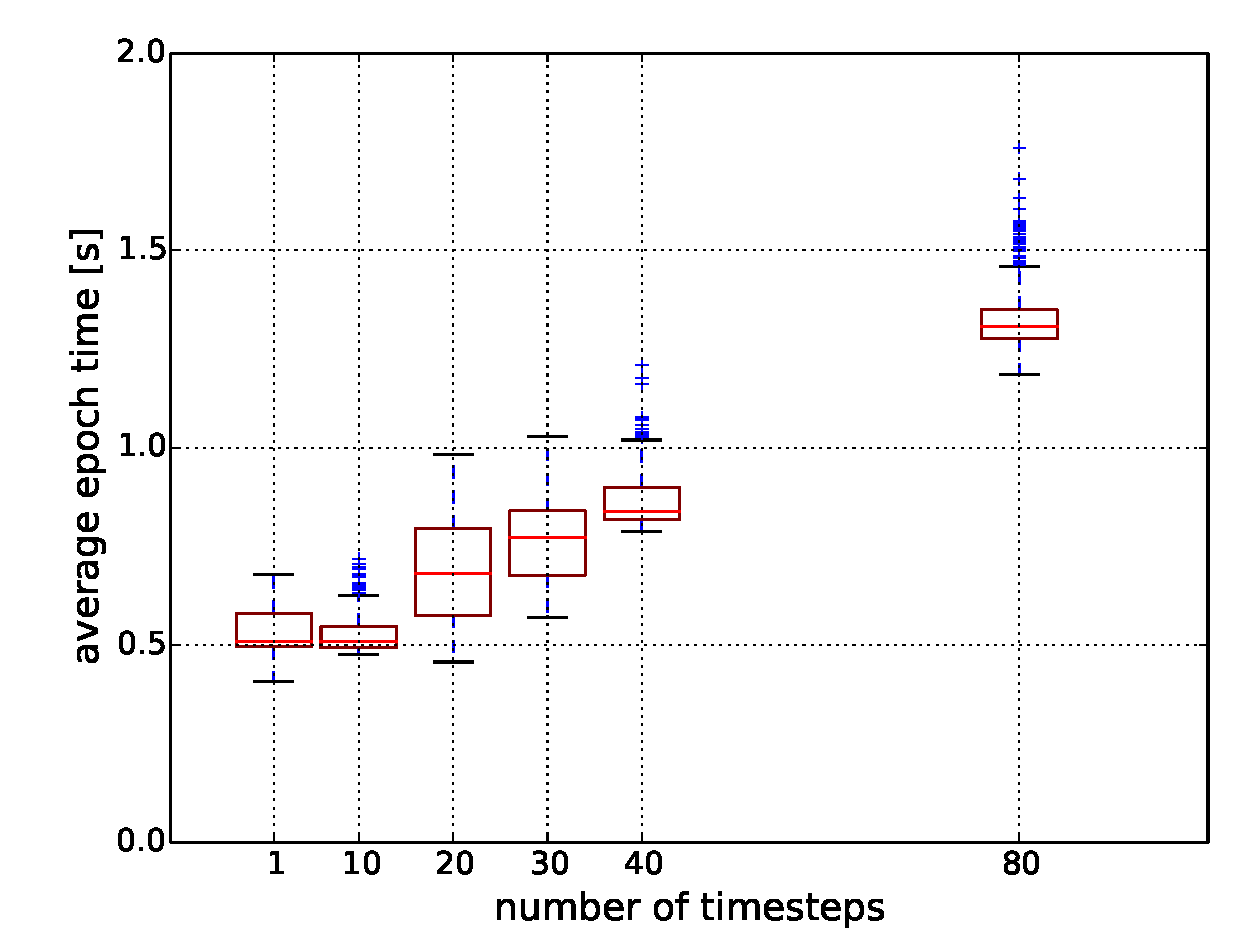
\includegraphics[width=1.0\textwidth]{cl_ts_time_boxplot}
  \caption{Number of simulation timesteps: influence on the accuracy and training time}
  \label{fig:ts_time_boxplot}
\end{figure}

\subsection{Analysis of Used Sensor Types} \label{ssec:analysis_of_used_sensor_types}

\begin{figure}[H]
  \centering
  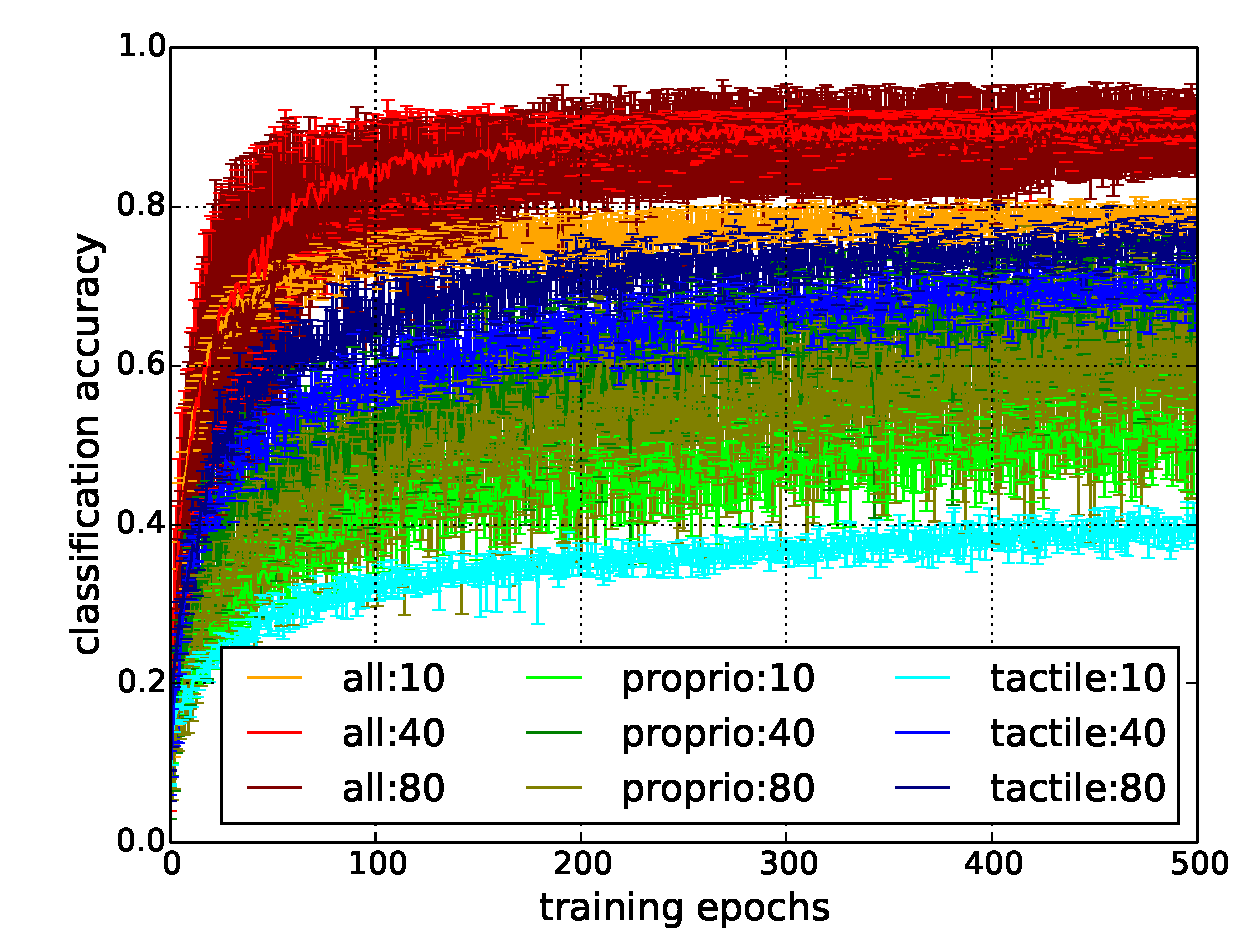
\includegraphics[width=1.0\textwidth]{cl_sen_vs_epoch}
  \caption{bla}
  \label{fig:sen_vs_epoch}
\end{figure}

\begin{figure}[H]
  \centering
  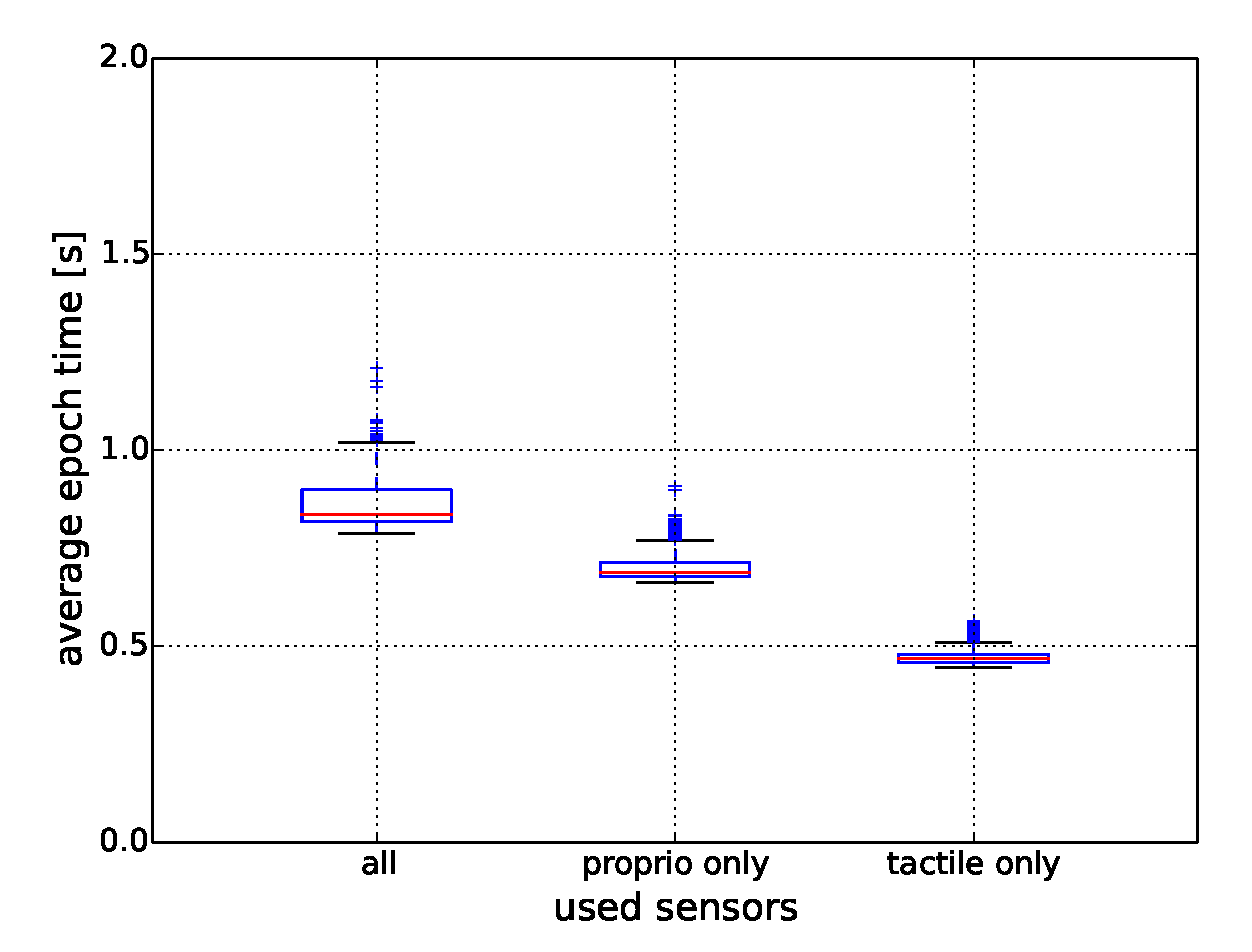
\includegraphics[width=1.0\textwidth]{cl_sen_time}
  \caption{bla}
  \label{fig:sen_time}
\end{figure}


\section[Terrain Classification Using Network Pruning]{Terrain Classification Using Network Pruning} \label{sec:pa_amter}

\begin{figure}[H]
  \centering
  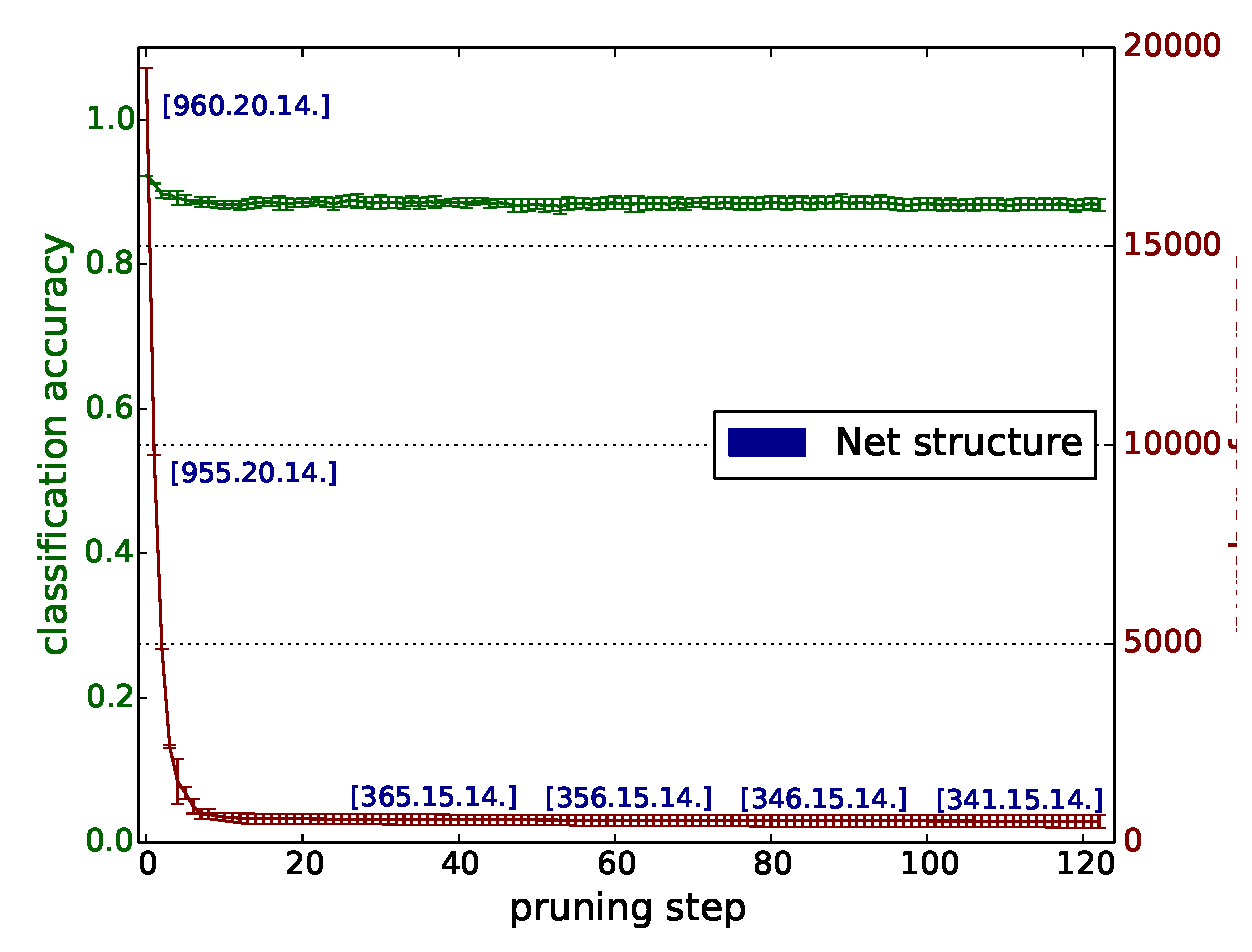
\includegraphics[width=1.0\textwidth]{pa_result_amter_nn}
  \caption{Pruning Algorithm Results on AMTER Dataset. No noise.}
  \label{fig:pa_result_amter}
\end{figure}

\begin{figure}[H]
  \centering
  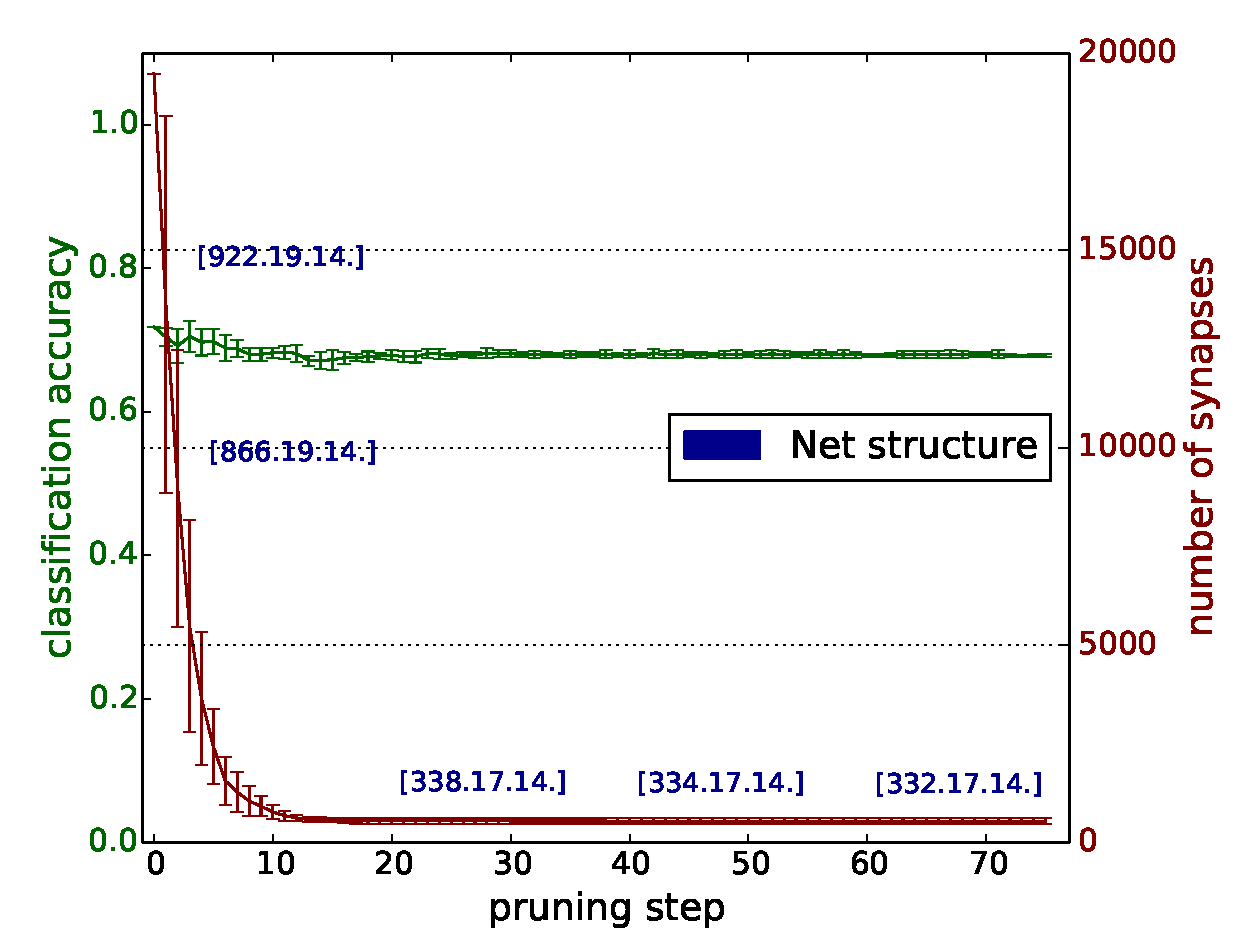
\includegraphics[width=1.0\textwidth]{pa_result_amter_noisy}
  \caption{Pruning Algorithm Results on AMTER Dataset. Noisy.}
  \label{fig:pa_result_amter_noisy}
\end{figure}

\begin{figure}[H]
  \centering
  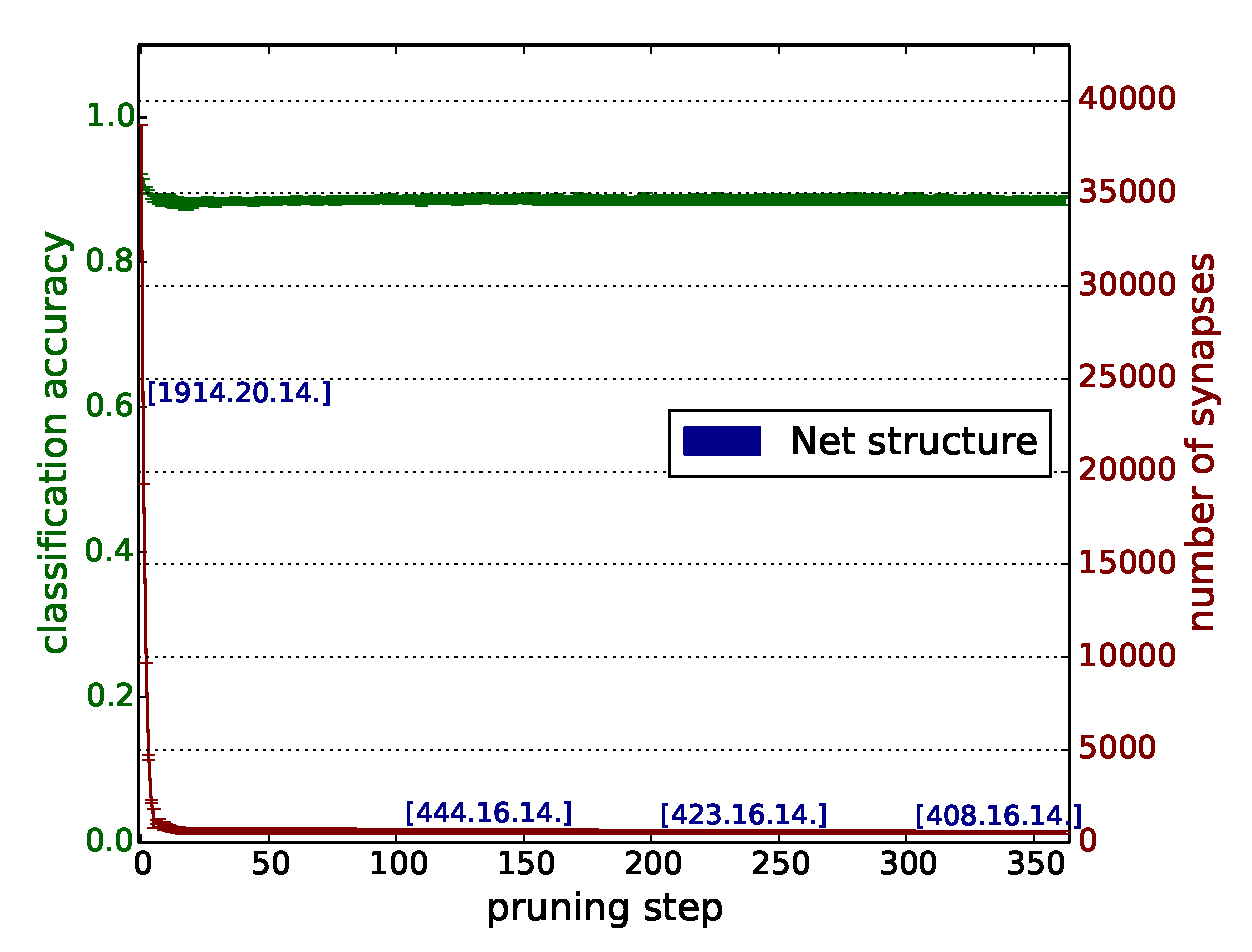
\includegraphics[width=1.0\textwidth]{pa_result_amter_ts80}
  \caption{Pruning Algorithm Results on AMTER Dataset. 80 timesteps.}
  \label{fig:pa_result_amter_80}
\end{figure}

\begin{figure}[H]
  \centering
  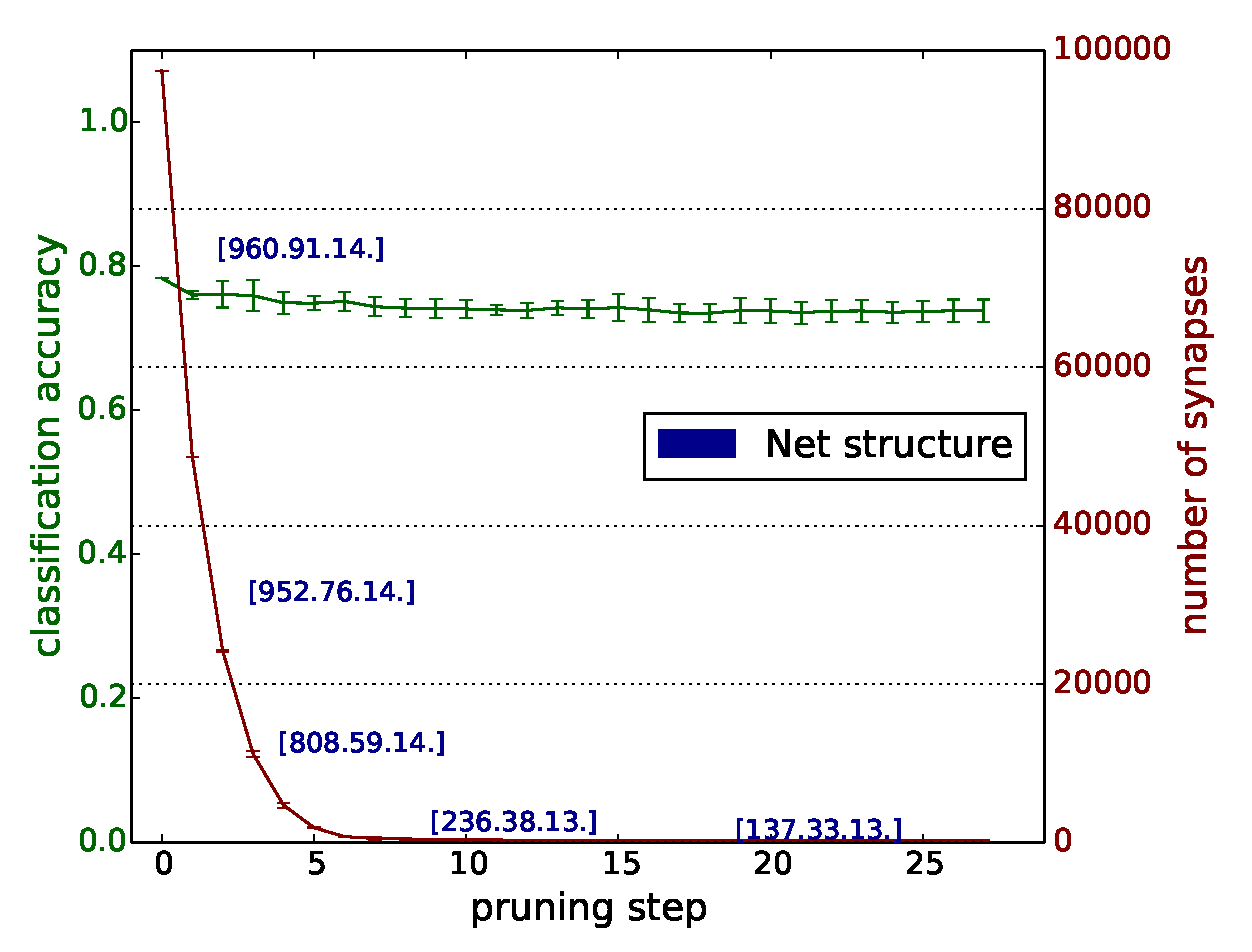
\includegraphics[width=1.0\textwidth]{pa_result_amter_st100}
  \caption{Pruning Algorithm Results on AMTER Dataset. 100 hidden neurons.}
  \label{fig:pa_result_amter_st100}
\end{figure}

\begin{figure}[H]
  \centering
  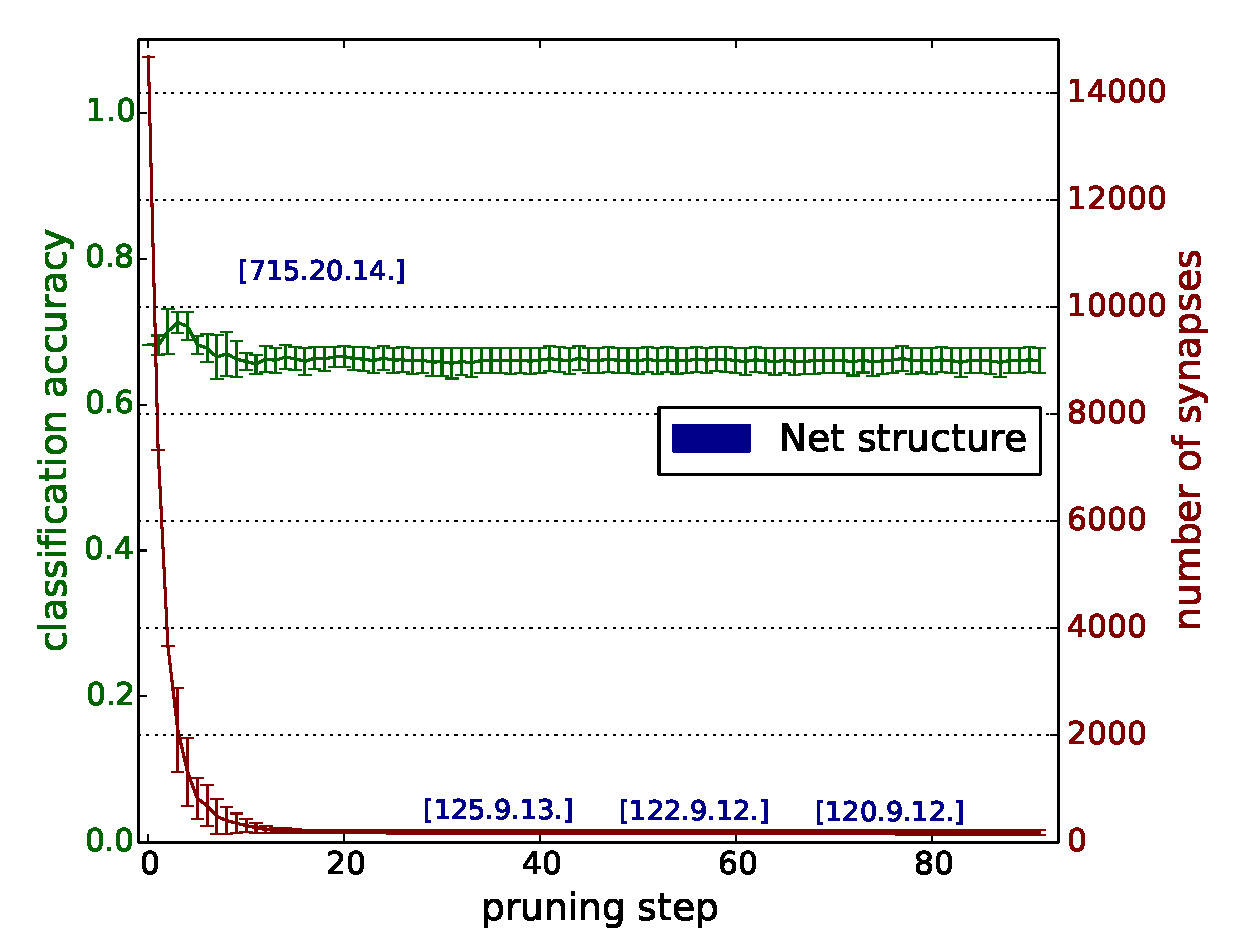
\includegraphics[width=1.0\textwidth]{pa_result_amter_angle}
  \caption{Pruning Algorithm Results on AMTER Dataset. Proprioceptive sensors only.}
  \label{fig:pa_result_amter_angle}
\end{figure}

\begin{figure}[H]
  \centering
  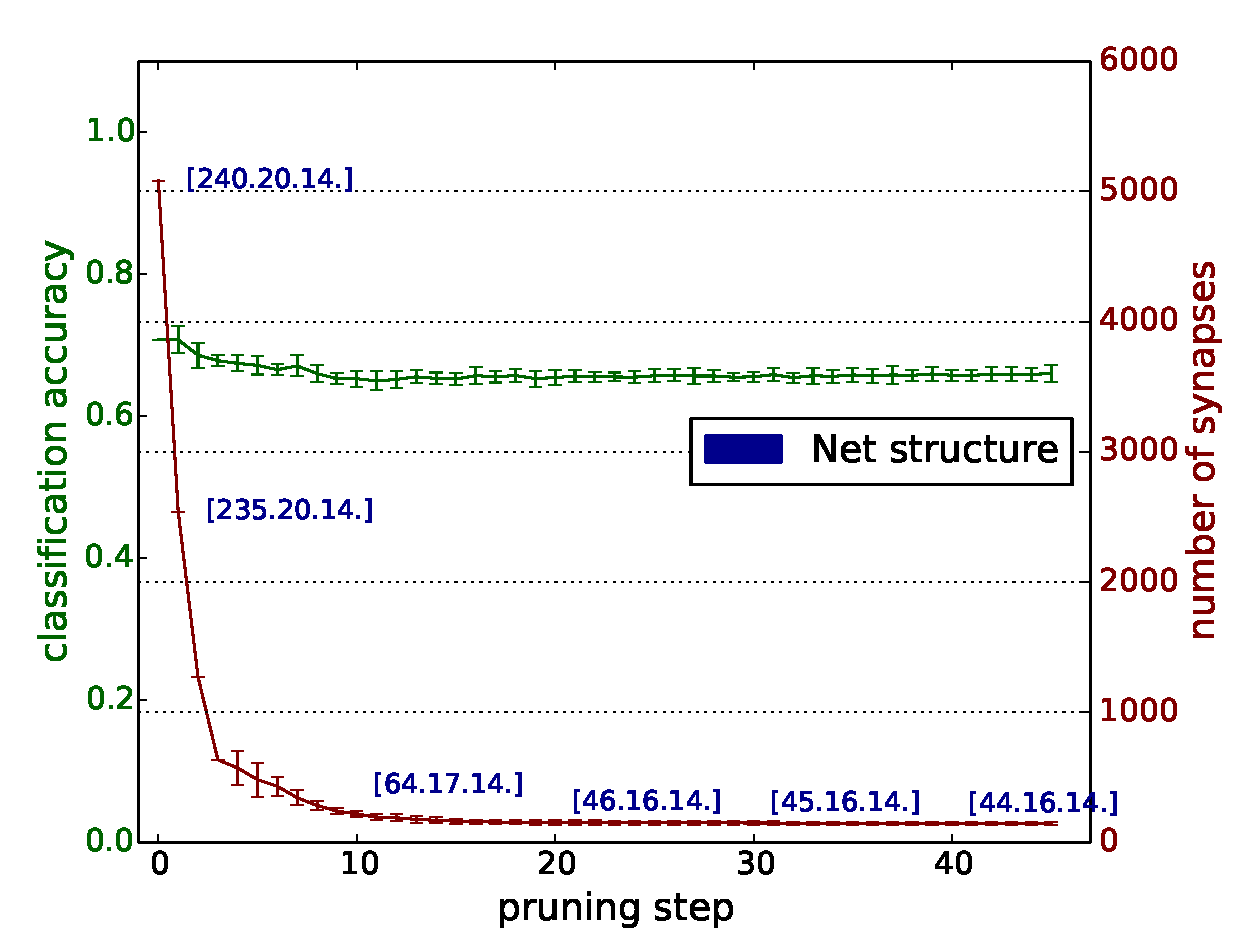
\includegraphics[width=1.0\textwidth]{pa_result_amter_foot}
  \caption{Pruning Algorithm Results on AMTER Dataset. Tactile sensors only.}
  \label{fig:pa_result_amter_foot}
\end{figure}

\begin{figure}[H]
  \centering
  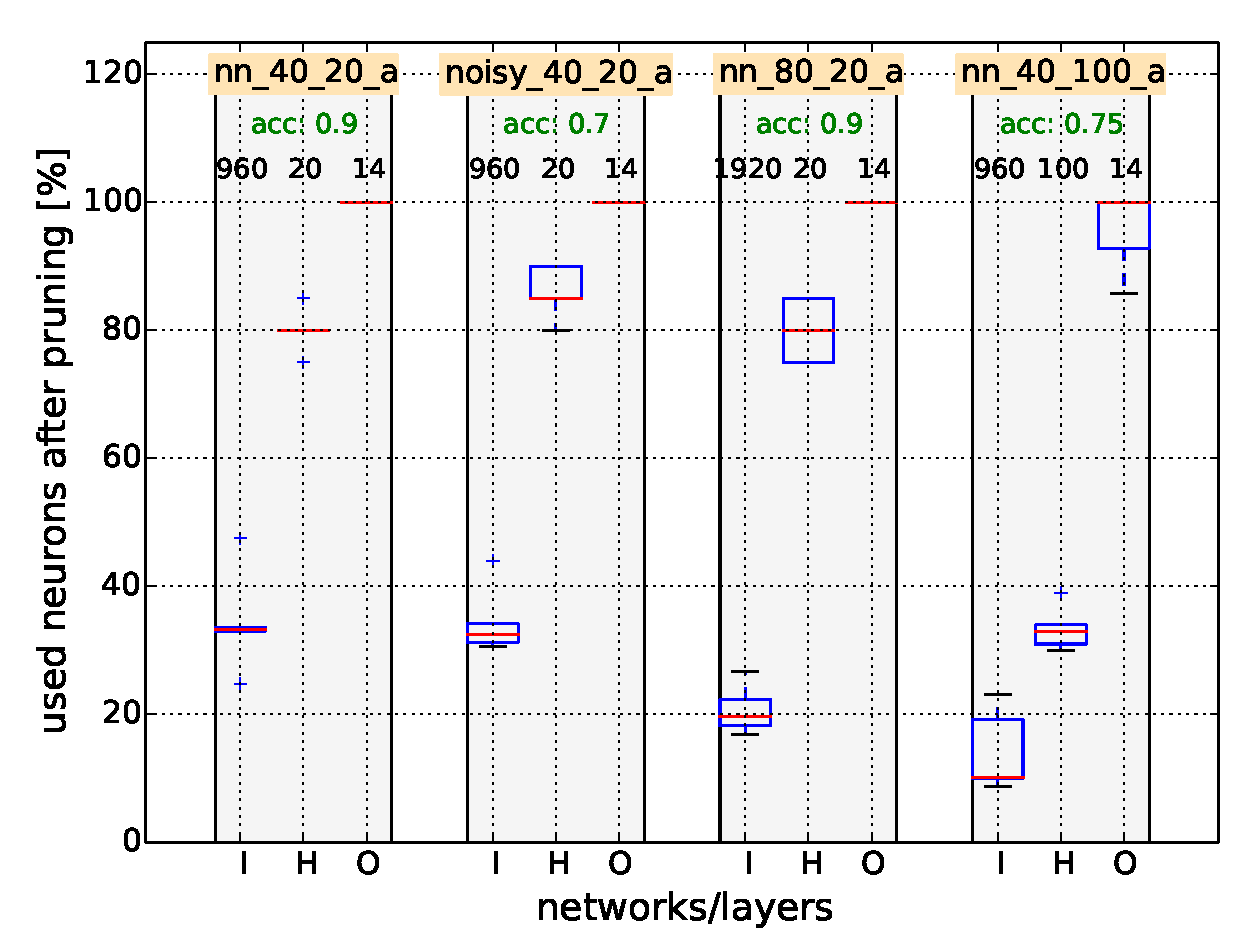
\includegraphics[width=1.0\textwidth]{pa_result_amter_used_neurons_allsen}
  \caption{Pruning Algorithm Results on AMTER Dataset. Used neurons allsen.}
  \label{fig:pa_amter_used_neurons_allsen}
\end{figure}

\begin{figure}[H]
  \centering
  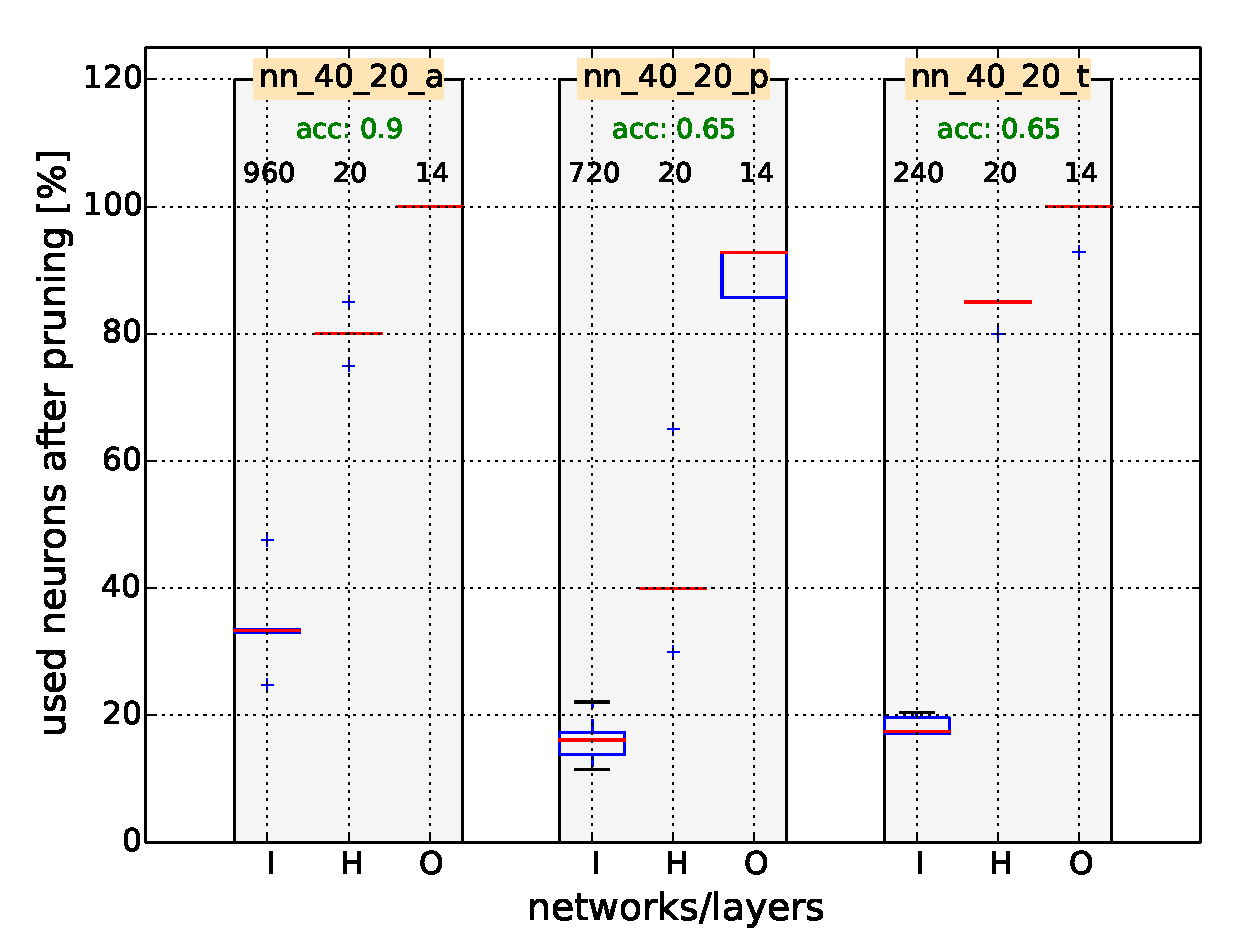
\includegraphics[width=1.0\textwidth]{pa_result_amter_used_neurons_ptasen}
  \caption{Pruning Algorithm Results on AMTER Dataset. Used neurons ptasen.}
  \label{fig:pa_amter_used_neurons_ptasen}
\end{figure}

\begin{figure}[H]
  \centering
  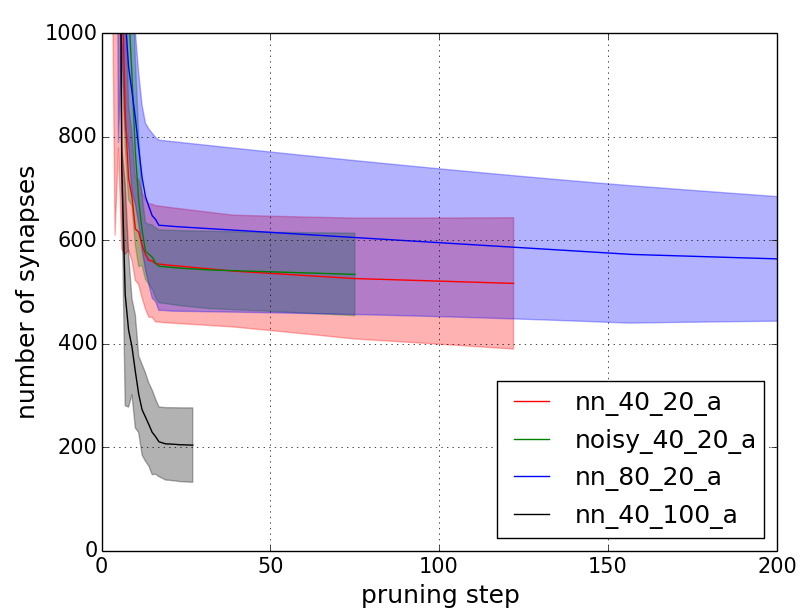
\includegraphics[width=1.0\textwidth]{pa_amter_synapses_allsen.png}
  \caption{Pruning Algorithm Results on AMTER Dataset. Synapses allsen.}
  \label{fig:pa_amter_synapses_allsen}
\end{figure}

\begin{figure}[H]
  \centering
  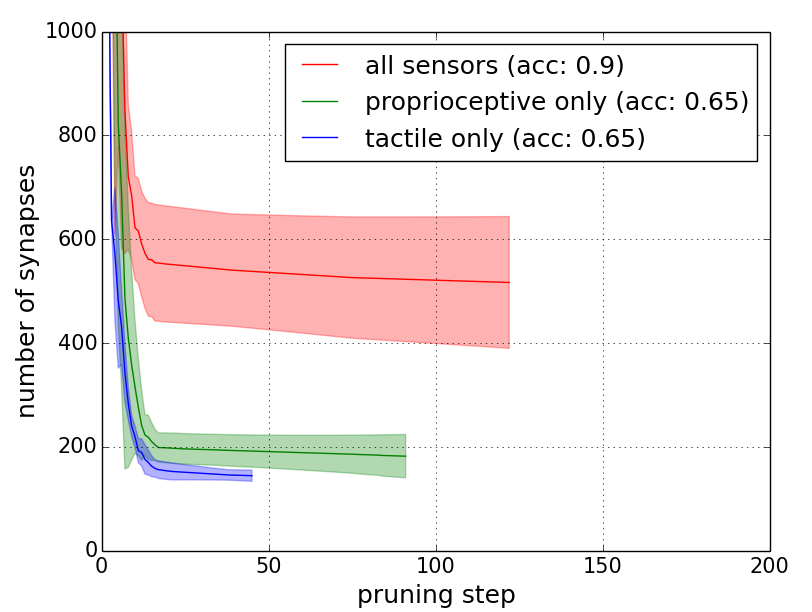
\includegraphics[width=1.0\textwidth]{pa_amter_synapses_ptasen.png}
  \caption{Pruning Algorithm Results on AMTER Dataset. Synapses ptasen.}
  \label{fig:pa_amter_synapses_ptasen}
\end{figure}

\subsection{Feature Selection for Terrain Classification} \label{ssec:pa_amter_feature_selection}

\begin{figure}[H]
  \centering
  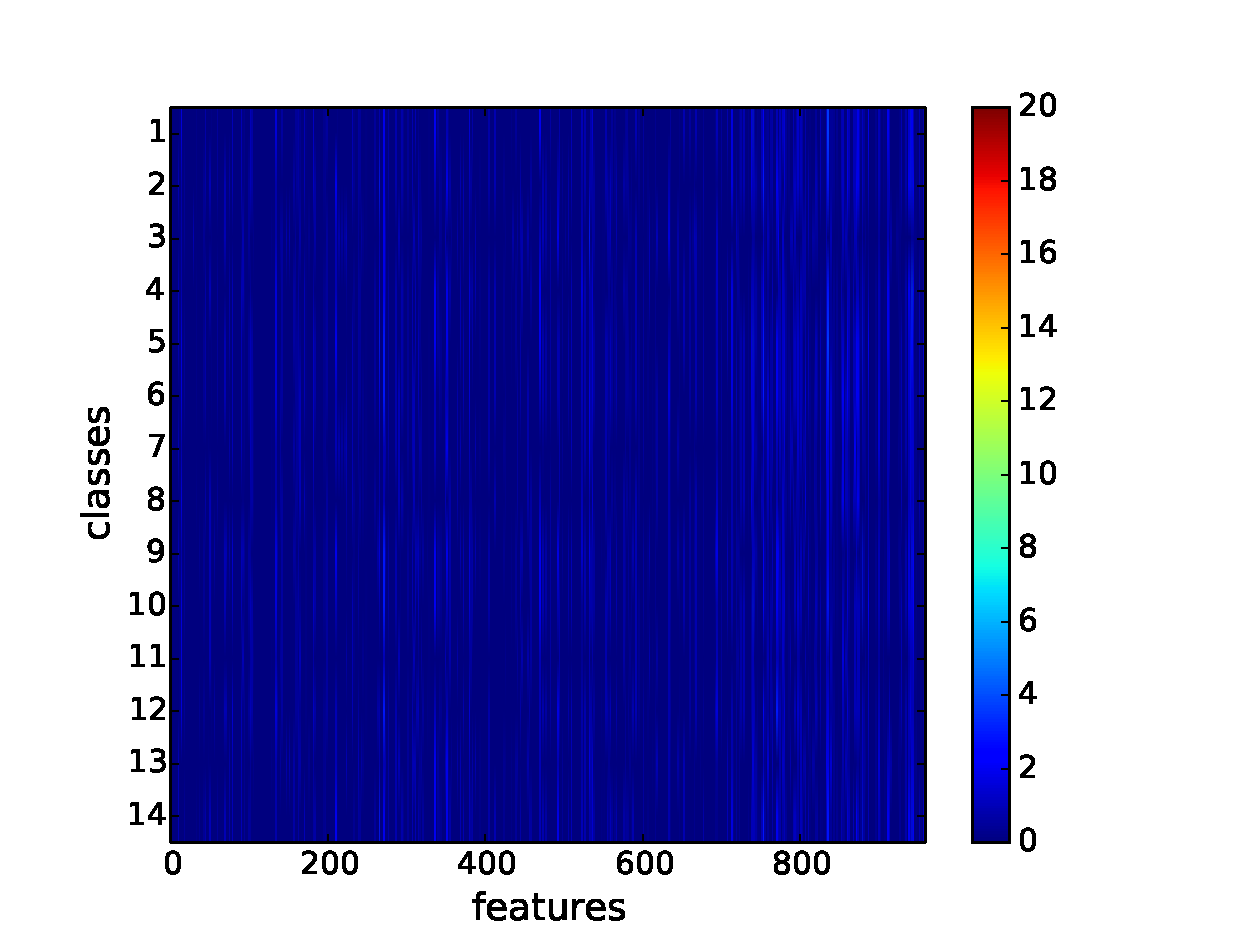
\includegraphics[width=1.0\textwidth]{fs_n_syn_to_hidden_by_class}
  \caption{Pruning Algorithm Results on AMTER Dataset. N synapses connected to the hidden layer, by class.}
  \label{fig:pa_amter_n_syn_to_hidden_by_class}
\end{figure}

\begin{figure}[H]
  \centering
  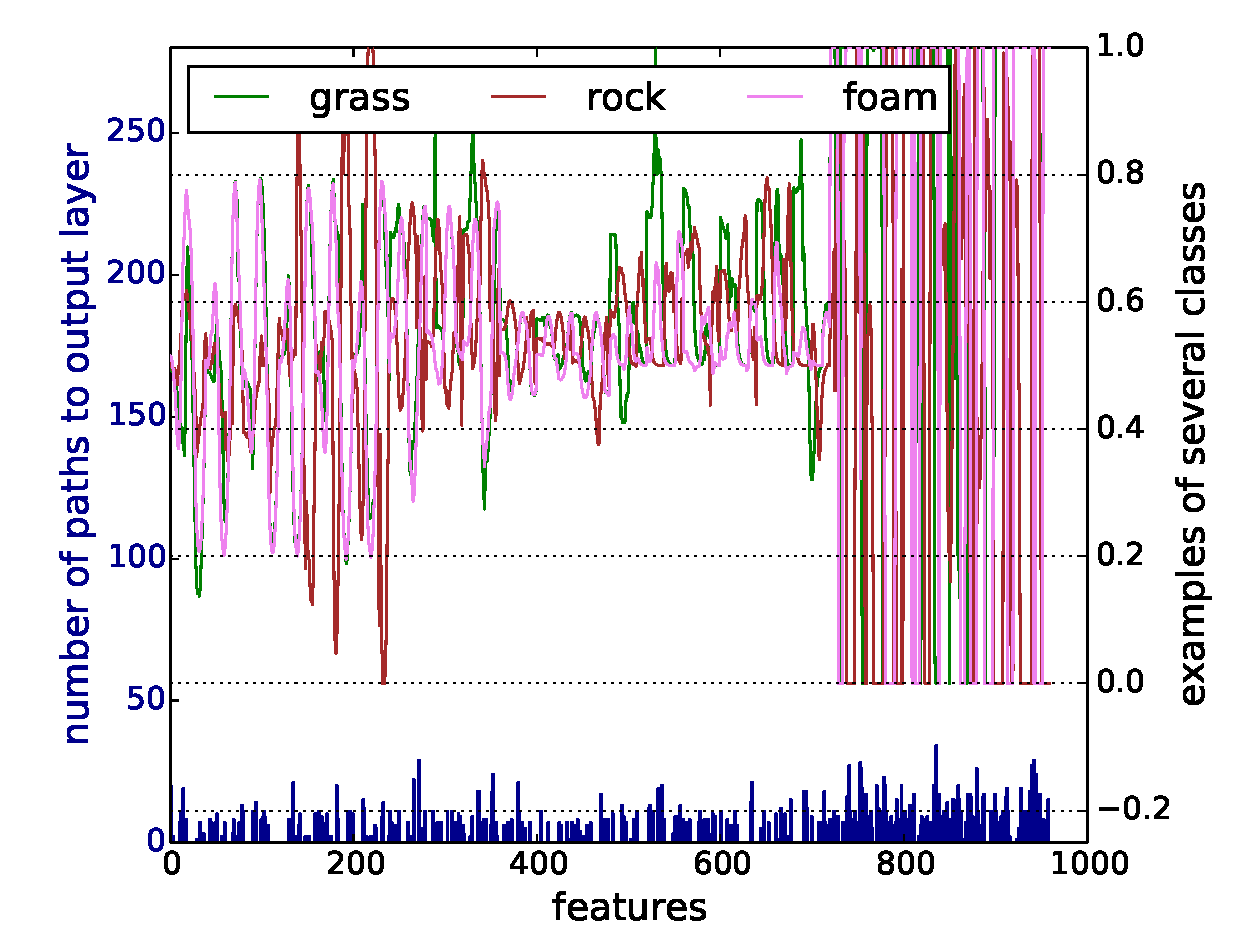
\includegraphics[width=1.0\textwidth]{fs_n_paths_to_output}
  \caption{Pruning Algorithm Results on AMTER Dataset. N synapses connected to the hidden layer, by class.}
  \label{fig:pa_amter_n_syn_to_hidden_by_class}
\end{figure}

\begin{figure}[H]
  \centering
  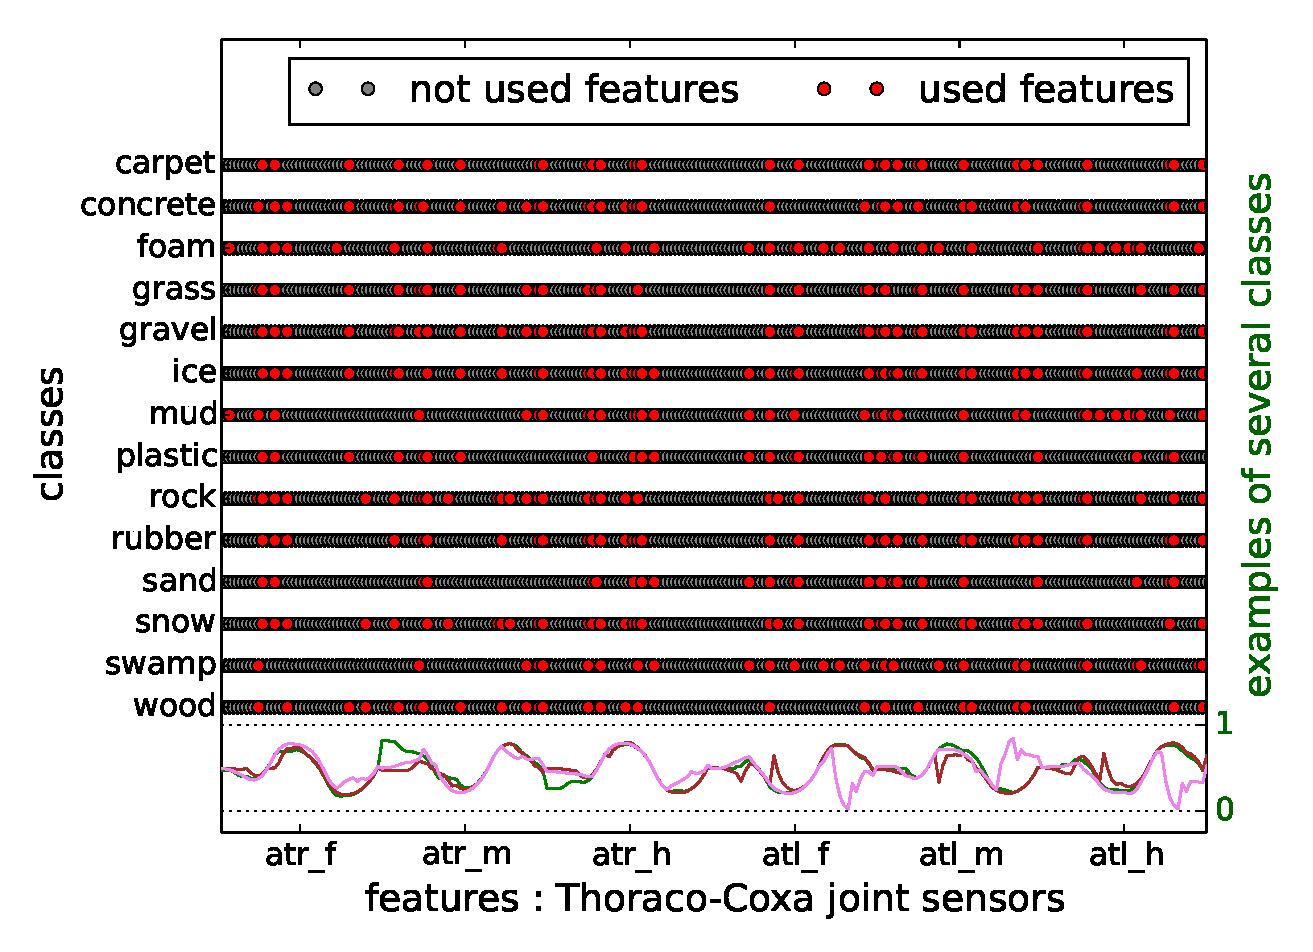
\includegraphics[width=1.0\textwidth]{fs_used_features_thoraco}
  \caption{Pruning Algorithm Results on AMTER Dataset. Used features thoraco.}
  \label{fig:pa_amter_used_features_thoraco}
\end{figure}

\begin{figure}[H]
  \centering
  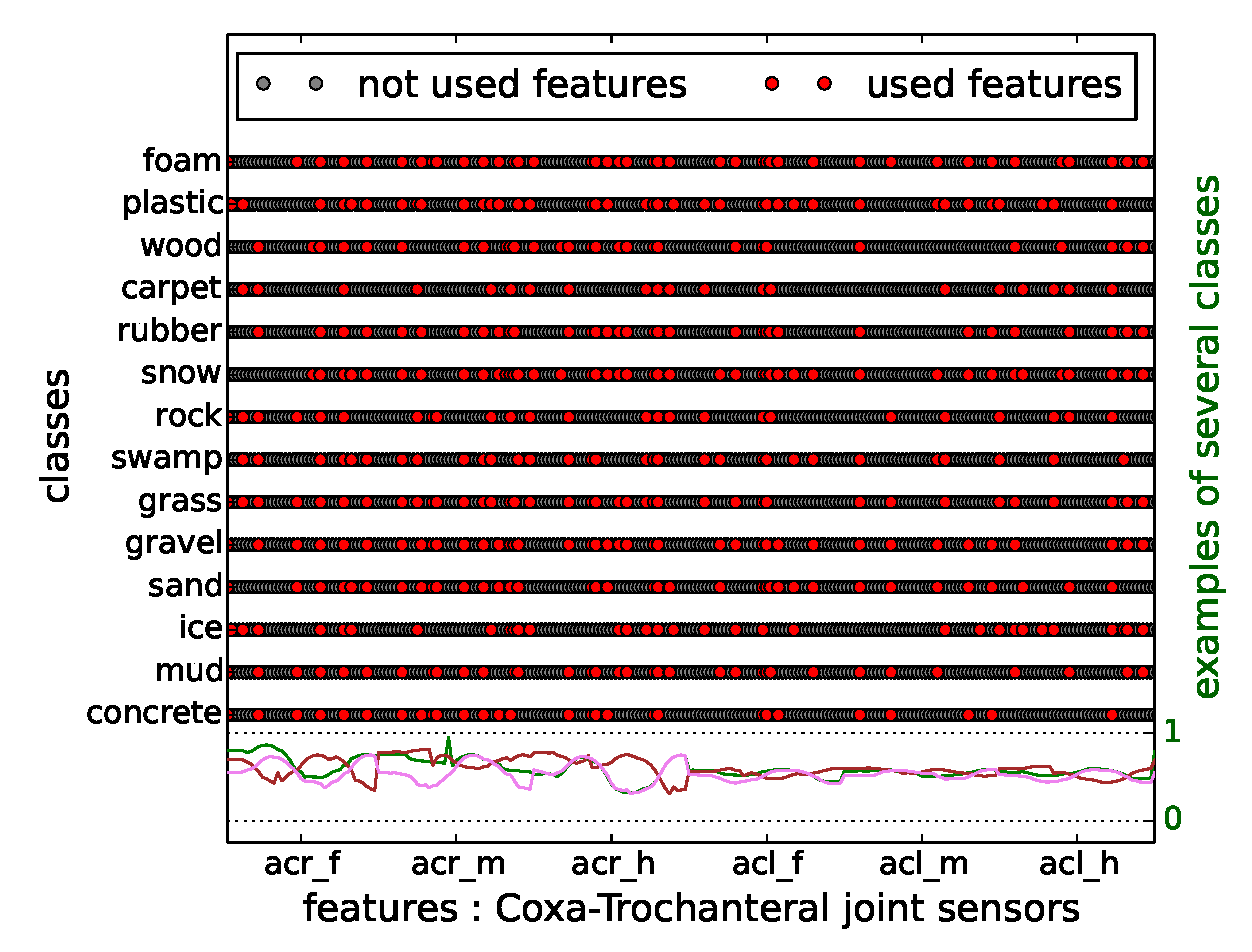
\includegraphics[width=1.0\textwidth]{fs_used_features_coxa}
  \caption{Pruning Algorithm Results on AMTER Dataset. Used features coxa.}
  \label{fig:pa_amter_used_features_coxa}
\end{figure}

\begin{figure}[H]
  \centering
  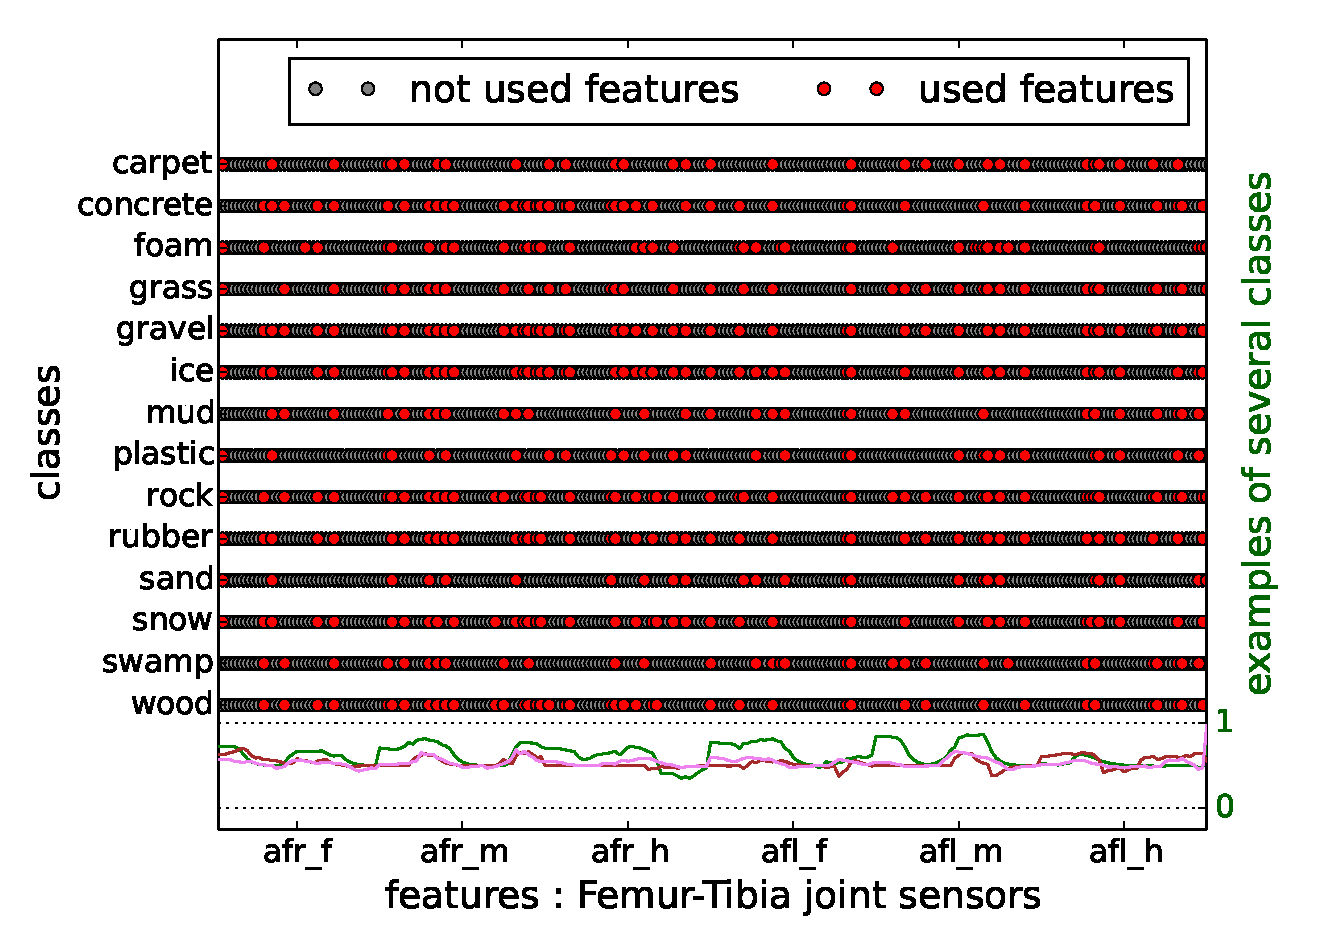
\includegraphics[width=1.0\textwidth]{fs_used_features_femur}
  \caption{Pruning Algorithm Results on AMTER Dataset. Used features femur.}
  \label{fig:pa_amter_used_features_femur}
\end{figure}

\begin{figure}[H]
  \centering
  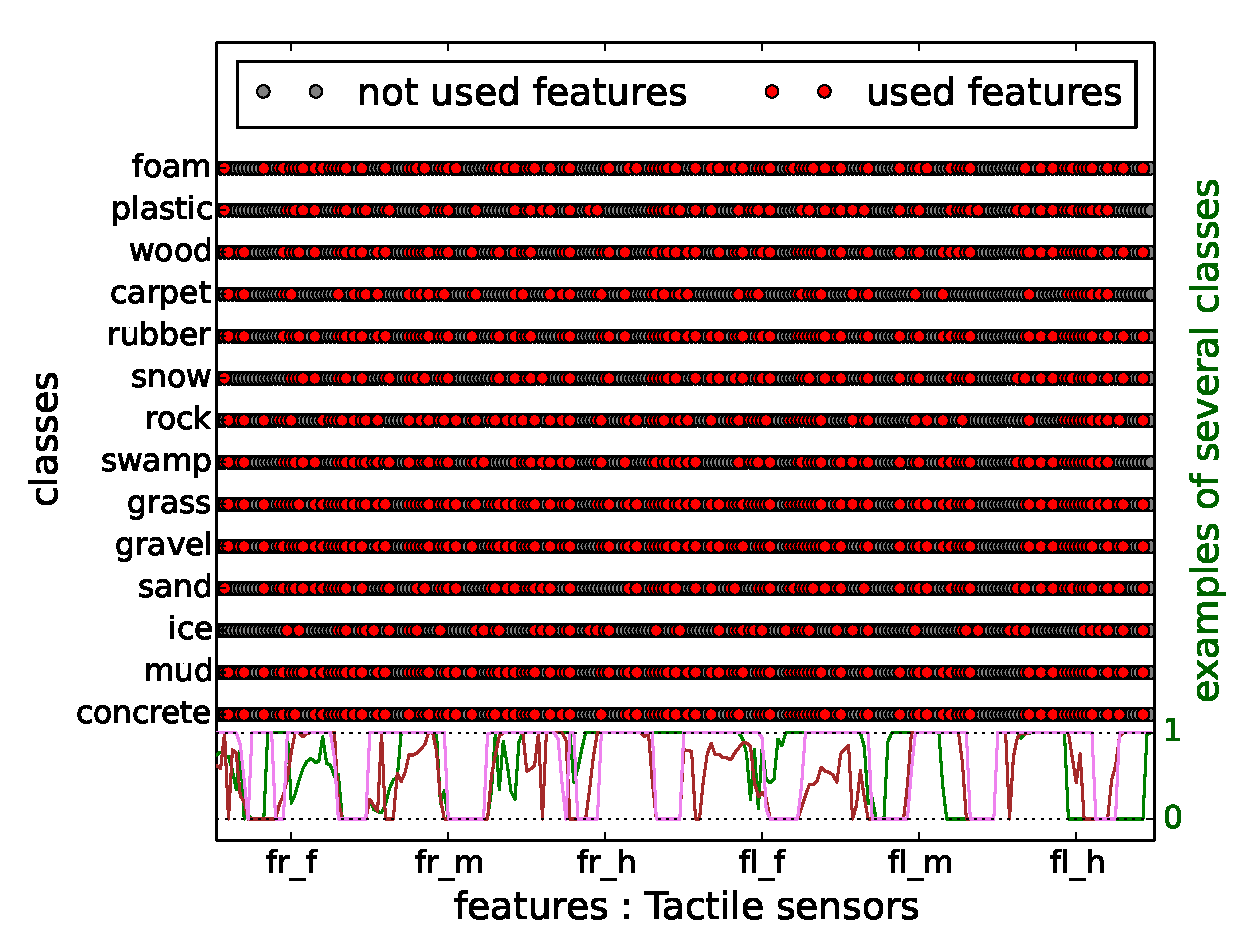
\includegraphics[width=1.0\textwidth]{fs_used_features_tactile}
  \caption{Pruning Algorithm Results on AMTER Dataset. Used features tactile.}
  \label{fig:pa_amter_used_features_tactile}
\end{figure}

evaluation (tables and figures) of classification:
\begin{itemize}
\item various terrain noise standard deviation values
\item various signal noise standard deviation values
\item various sensors on network input (only foot, only angle...)
\item various timesteps used as one sample (-> time needed for detection)
\item various number of detected terrains as outputs
\item various network structures
\item various training parameters (epochs, learning rate, batch size...)
\end{itemize}


evaluation of neural nets as a classifier:
\begin{itemize}
\item comparison to other classifiers on the same data, classifiers are ready provided by sknn library
\end{itemize}

evaluation of proprioception sensing against other methods (visual, haptic, laser...):
\begin{itemize}
\item comparison to the results from the literature
\end{itemize}

evaluation of the pruning algorithm:
\begin{itemize}
\item various starting structures, ends up with the same minimal-optimal structure?
\item various noise types, same minimal structure?
\item speed comparisons of the fully-connected vs. pruned structure
\item further analysis:
 \begin{itemize}
 \item which sensors are redundant/crucial
 \item which sensors are important for which terrain
 \item comments on the minimal structure and benefits of having it
 \end{itemize}
\end{itemize}
10-15 pages (many figures, tables)
